\documentclass[uplatex]{sumiilab-paper}
%% platex を使う場合:
%% \documentclass{sumiilab-paper}

\usepackage[dvipdfmx]{graphicx} % 各種形式の画像を簡単にincludeできます
\usepackage{amsmath,amssymb} % 数式
\usepackage{bm}
\usepackage{mathtools} % 数学記号
\usepackage{stmaryrd}
\usepackage{cite} % 引用
\usepackage{enumitem} % リスト環境
\usepackage{bussproofs} % 証明器

\usepackage{listings, jvlisting} % ソースコード
\usepackage{amsthm} % 定理環境

\usepackage{url}
\usepackage{comment} % 追加

%% =========================================
%% 定理環境の設定
%% =========================================
\newtheoremstyle{mystyle}% name
{}% space above
{}% space below
{\normalfont}% body font
{}% indent amount
{\bfseries}% theorem head font
{ }% punctuation after theorem head
{4pt}% space after theorem head (default: 5pt)
{\thmname{#1}\thmnumber{#2}\thmnote{\hspace{2pt}(#3)}}% theorem head spec

\theoremstyle{mystyle}
\newtheorem{definition}{定義}
\newtheorem{theorem}[definition]{定理}
\newtheorem{corollary}[definition]{系}
\newtheorem{proposition}[definition]{命題}
\newtheorem{lemma}[definition]{補題}
\newtheorem{example}[definition]{例}
\newtheorem{assumption}[definition]{仮定}
\newtheorem{axiom}[definition]{公理}
\renewcommand{\proofname}{\bf{証明}}
\numberwithin{definition}{chapter} % 定義1.1のように表示

%% ソースコードのキャプション名
\renewcommand{\lstlistingname}{ソースコード}
%% ===============================================
%% 論文の表紙に表示される情報
%% ===============================================

% 論文の年度と種類
\paper{2023 年度 卒業論文}% 学部生
%\paper{20XX 年度 修士論文}% 修士

% 論文のタイトル
\title{OCamlにおけるEmbedding by Unembedding}

% 学籍番号と著者のお名前
\author{C0TB2512 類家 健永}

% 著者の所属
\institute{東北大学 工学部\\電気情報物理工学科}% 学部生
%\institute{東北大学 大学院情報科学研究科\\情報基礎科学専攻}% 修士

% 指導教員のお名前
\supervisor{住井 英二郎 教授}% 指導教員
\subsupervisor{松田 一孝 准教授}% 論文指導教員(省略可)

% 論文発表日時
\date{2024 年2月28日 \quad 14:00--14:30}
% 発表場所
\venue{青葉山キャンパス 電気系3号館 206セミナー室}

%% ===============================================
%% ソースコードの設定
%% ===============================================

% プログラミング言語と表示するフォント等の設定
\lstset{
  language={[Objective]Caml},% プログラミング言語
  basicstyle={\ttfamily\small},% ソースコードのテキストのスタイル
  keywordstyle={\bfseries},% 予約語等のキーワードのスタイル
  commentstyle={},% コメントのスタイル
  stringstyle={},% 文字列のスタイル
  frame=trlb,% ソースコードの枠線の設定 (none だと非表示)
  numbers=left,% 行番号の表示 (none だと非表示)
  numberstyle={\footnotesize},% 行番号のスタイル
  xleftmargin=15pt,% 左余白
  xrightmargin=5pt,% 右余白
  keepspaces=true,% 空白を維持する
  mathescape,% $ で囲った部分を数式として表示する ($ がソースコード中で使えなくなるので注意)
  % 手動強調表示の設定
  moredelim=[is][\bfseries]{@*}{*@},
  moredelim=[is][\itshape]{@/}{/@},
  captionpos=b
}
\lstMakeShortInline[columns=fullflexible]|% 本文中にコードを|foo|の形式で書くことができます

%% ===============================================
%% 論文中で使う記号とかのマクロ定義
%% ===============================================

%% 論文中で繰り返し使う記号は次のように「マクロ」として実装しておくと良い。
%% TeX ソース中で \BOOL と書くと、\texttt{Bool} に置き換えてくれる。
%% フォントを変え忘れたりするリスクが減るし、あとから記号を変更するのも楽になる。

\newcommand{\bkeyword}[1]{\ensuremath{\mathbf{#1}}}
\newcommand{\BOOL}{\bkeyword{Bool}}
\newcommand{\TRUE}{\bkeyword{true}}
\newcommand{\FALSE}{\bkeyword{false}}
\newcommand{\IF}{\bkeyword{if}}
\newcommand{\THEN}{\bkeyword{then}}
\newcommand{\ELSE}{\bkeyword{else}}

\begin{document}
\frontmatter% ここから前文

\maketitle

\begin{abstract}
埋め込み領域特化言語は他の言語のライブラリの形で実装された言語であり、ホスト言語の機能やエコシステムを利用可能であるという利点がある。
埋め込み領域特化言語の実装方式の一つにEmbedding by Unembedding (EbU)がある。
EbUは双方向変換や漸増計算など複雑な意味の言語を、高階抽象構文を用いて実装することを可能とする。
元のEbUはHaskellで実装されている。
しかし、型クラス、GADT、型族、高階多相などの高度な機能が用いられているため、他の関数プログラミング言語での実現方式は明らかでなかった。
本研究ではOCamlにおけるEbUの実現方式を示し、例を通してその有用性を評価する。
\end{abstract}

\tableofcontents% 目次

\mainmatter% ここから本文

\chapter{序論}
領域特化言語は特定の問題を解決するために、その問題の領域に特化した言語である。特に他の言語のライブラリの形で実装された領域特化言語は埋め込み領域特化言語と呼ばれる。
埋め込み領域特化言語はその実装方式から、他の言語のユーザがホスト言語の機能やエコシステムを利用可能であるという利点がある。\\
% しかし、言語の変数の取り扱いは面倒であり、変数束縛の強引な実装はエラーが発生しやすくなる。\\
 埋め込み実装においては変数の取り扱いが問題となる。
例えば、変数をそのまま文字列で表現するような素朴な実装は煩雑であり誤りやすい。
解決策の一つにHigher-Order Abstract Syntax(HOAS)\cite{Church_1940,huet_hoas,miller_hoas,phenning_hoas}がある。
HOASはゲスト言語の変数束縛をホスト言語の関数で表現する。
HOASはユーザが利用しやすい一方、一部の言語については開いた式の意味をホスト言語の関数として表現することが難しいためHOASの利用が自明ではない。
例えば、双方向変換や増分計算、可逆計算がこれに該当する。\\
 埋め込み領域特化言語の実装方式の一つにEmbedding by Unembedding(EbU)\cite{matsuda2023embedding}がある。
EbUは開いた式の意味をホスト言語の関数として変換する{\tt lift}処理が提供されており、{\tt lift}処理によりHOASを用いて双方向変換や増分計算などを表現可能にする。
元のEbUはHaskellで実装されている。
しかし、EbUの現在の実装はHaskellの型クラス、GADT、型族、高階多相などの高度な機能が用いられているため、他の関数型プログラミング言語での実装方式は明らかではない。\\
 本研究では、EbUをユーザビリティを維持しつつ実装するにはどのような言語機能が重要となるのかを明らかにするための最初のステップとして、他のメジャーな関数型プログラミング言語であるOCamlでEbUの実装を行う。
% GADTを利用している箇所はそのままに、型族や型クラス、高階型オペレータを利用している箇所についてはmodule/ファンクタ機能を用いる。
そして、増分計算の例により、その有用性を評価する。\\
 本研究の貢献は以下である。
\begin{itemize}
  \item EbUを他の関数型プログラミング言語で実装するときの問題点の特定(3.1節)
  \item OCamlでの新しい実装方式の提案(3.3節)
  \item 増分計算の例により、OCaml版EbUでもユーザビリティが維持されていることを確認(4章)
\end{itemize}
また、結論(6章)を述べる前に、関連研究(5章)について議論を行う。


%% 参考文献は \cite{ID} とします(ID は refs.bib 内で文献につけた識別子)
%% BibTeX の使い方などは各自調べて下さい。
%% 序論とか結論とか \cite{Pierce:TypeSystems}

\chapter{準備}
本章では、EbUを実装するにあたり、その基礎となる知識の準備を行う。
EbUはユーザが扱うHOASと意味領域上で動作する意味関数を接続するフレームワークとして機能する。
したがって、本章ではHOAS、Embedding by Unembeddingについて説明する。
2.1節ではHOASを、2.2節ではEmbedding by Unembeddingを扱う。

% \section{De Bruijn項}
% De Brujin項はEbUの基礎となっているUnembeddingで利用される項の表現方法である\cite{Pierce:TypeSystems}。
% EbUでは直接De Bruijn項を扱うことはない。
% 項の開いた式を考える際に、便宜上De Bruijn項を利用する。
% したがって、ここではDe Bruijn項がどのような項の表現方法であるかを簡潔に述べる。\\
%  De Bruijn項は変数名を扱わない項の表現方法一つである。
% De Bruijn項は項に出現する変数を名前を介して参照するのではなく、束縛子を直接示すことで参照する。
% 束縛子の指定には自然数が用いられ、変数は束縛子からの深さで表現される。\\
%  例えば、型無しλ計算では恒等関数をラムダ抽象を用いて$\lambda x.~x $
% と表現する。$\lambda x$は$x$を指している。したがって、恒等関数では$x$は深さが0であるため、De Bruijn項では
% $\lambda.~0 $と表現される。
% 変数が複数ある場合も同様である。$\lambda x.\lambda y.~x~(y~x)$は$\lambda.\lambda.~1~(0~1)$に対応する。\\
 
%  自由変数を含む項に対しては少し注意が必要である。例えば、関数適用の項は$x~y$と表現される。
% この項はラムダ抽象が含まれないため、そのままではde Bruijn項として表現できない。
% そこで、次の環境をあらかじめ与える。
% \begin{align}
% \begin{array}{rcl@{\qquad\qquad}r}\notag
%     \Gamma ~=~ x &\mapsto& 4 \\
%                y &\mapsto& 3 \\
%                z &\mapsto& 2 \\
%                a &\mapsto& 1 \\
%                b &\mapsto& 0
% \end{array}
% \end{align}

%  ラムダ抽象が含まれない項も、この環境に従って表現できる。関数適用の項は$4~3$と表現される。
% もちろん、自由変数と束縛変数を両方含む項も表現ができ、$\lambda w.~y~w$は$\lambda.~4~0$と表現される。
% ここで、$y$を示すインデックスが一つずれるが、これは束縛子の情報が環境に追加されたために発生する。

% 本節では、BNF によるプログラミング言語の構文の書き方を紹介する。
% 構文木の書き方は一つというわけではないので、幾つかのバリエーションを紹介する。
% どの方法が良いと思うかは、個人の好みに依るところなので、好きなものを使えば良いと思う。

% まず、次の方法では、array 環境を使って、BNF を書いている。
% array 環境は数式環境中で表のようなものを書くときに使う。
% 基本的に、table 環境と使い方は同じである。
% \[
% %% 空白を明示的に開けるときは "\," "\ " "~" "\quad" "\qquad" などを使う。
% %% 空白の幅は "\qquad" > "\quad" > "~" = "\ " > "\," の順で大きい。
% %% "~" と "\ " は空白の代わりに改行を許すかどうかの違い("\ " だと改行される可能性がある)
% \begin{array}{rcl@{\qquad\qquad}r}
%   t & \Coloneqq & & \text{terms:} \\
%   & \mid & x & \text{variables} \\
%   & \mid & \lambda x.~t & \text{lambda abstraction} \\
%   & \mid & t_1~t_2 & \text{application} \\
%   & \mid & \TRUE & \text{true} \\
%   & \mid & \FALSE & \text{false} \\
%   & \mid & \IF~t_1~\THEN~t_2~\ELSE~t_3 & \text{if statement}
% \end{array}
% \]

% 他にも、次のように、align 環境を使っても、似たようなものを書くことができる。
% \begin{align}
%   t \Coloneqq & \tag*{terms:} \\
%   {}\mid{} & x \tag*{variables} \\
%   {}\mid{} & \lambda x.~t \tag*{lambda abstraction} \\
%   {}\mid{} & t_1~t_2 \tag*{application} \\
%   {}\mid{} & \TRUE \tag*{true} \\
%   {}\mid{} & \FALSE \tag*{false} \\
%   {}\mid{} & \IF~t_1~\THEN~t_2~\ELSE~t_3 \tag*{if statement}
% \end{align}
% array 環境を愚直に使う場合と比べて、式が中央揃えになるという点と、
% ``variables'' とかの説明が右端に来ている点が違う。
% 説明は tag* マクロで出しており、これはもともと式番号を指定するためのものなので、
% 若干使い方がおかしい気もするが、まぁ、いいだろう。
% 自分の好みの方を使うと良いだろう。

% BNF 全体を左揃えにしたいならば、次のように、flalign 環境を使うと良い。
% align 環境と違って、\verb|&| を余分に一つ付ける必要がある、ということに注意して欲しい(詳しくはソースコードを見よ)。
% \begin{flalign}
%   t \Coloneqq & & \tag*{terms:} \\ % & を余分に一つ付けること!
%   {}\mid{} & x \tag*{variables} \\
%   {}\mid{} & \lambda x.~t \tag*{lambda abstraction} \\
%   {}\mid{} & t_1~t_2 \tag*{application} \\
%   {}\mid{} & \TRUE \tag*{true} \\
%   {}\mid{} & \FALSE \tag*{false} \\
%   {}\mid{} & \IF~t_1~\THEN~t_2~\ELSE~t_3 \tag*{if statement}
% \end{flalign}

\section{HOAS}
Embedding by Unembedding(EbU)ではHigher-Order Abstract Syntax(HOAS)を用いて言語を埋め込む。
HOASとは変数束縛の表現方法の一つであり、変数束縛をホスト言語の関数で表す。
EbUでHOASを用いる理由は、埋め込み言語の利便性の向上のためである。
例えば、HOASはゲスト言語の変数をホスト言語の関数で管理するため、言語実装者が変数の名前管理をする必要がない。\\
 EbUではtagless-final style\cite{CARETTE_KISELYOV_SHAN_2009}によりHOASを埋め込む。
tagless-final styleはshallow embeddingの一種である。
% shallow embeddingは言語の言語要素を増やすことに有利ではあるが、解釈を増やすことは不得意とする埋め込みDSL実装方式である。
% tagless-final styleはshallow embeddingの利点はそのままに、解釈を増やすことに成功している。
tagless-final styleでは、ゲスト言語の式を多相型で表し、項および言語要素を抽象化し、解釈に応じて適切な実装を与える。\\
% \begin{align}
% &guestExp~::~(\{-lit-\} Int \rightarrow a) \rightarrow (\{-add-\} a \rightarrow a \rightarrow a) \rightarrow a \notag\\
% &guestExp~lit~add~=~add~(lit~3)~(add~(lit~4)~(lit~5)) \notag 
% \end{align}
% という多相型で表す。\\
% 多相型を用いることで、式に適切な関数を代入することで構文木をたどらずに解釈を増やせる。\\
% 例えば、$guestExp~id~(+)$とすることで通常の評価を行うことができ、$guestExp~show~(fun~n~m\rightarrow"("~++~n~++~"+"~++~m~++~")")$とすることで式の出力が可能となる。\\
% tagless-final styleはHOASとしての利点もある。例として、型なしラムダ計算をHOASで表す。型なしラムダ計算はHOASで
% \begin{align}
%   data~Exp~&where \notag \\
%   App~&::~Exp \rightarrow Exp \rightarrow Exp \notag \\
%   Lam~&::~(Exp \rightarrow Exp) \rightarrow Exp \notag
% \end{align}
% と表される。しかし、この方法では式を解釈する関数の記述が難しい。
% 例えば、$data~Val~=~VFun~(Val \rightarrow Val)$として、評価関数$eval~::~Exp \rightarrow Val$を定義する場合に評価の中で$Val \rightarrow Exp$という関数が必要となったり、元の計算体系で表現できない式を許すことがあったりする。
% tagless-final styleは、この問題を解決する手法でもある。同様の型なしラムダ計算において
% \begin{align}
%   class~Lam~e&~where \notag \\
%   app~&::~e \rightarrow e \rightarrow e \notag \\
%   lam~&::~(e \rightarrow e) \rightarrow e \notag
% \end{align}
% について、 
% \begin{align}
%   instance&~Lam~Val~where \notag \\
%   &app~(VFun~f)~x~=~f~x \notag \\
%   &lam~k~=~VFun~k \notag
% \end{align}
% のようにして、評価関数を定義できる。\\
 EbUはtagless-final styleとunembedding\cite{syntaxforfree_atkey,unembedding_atkey}を組み合わせたフレームワークであるため、tagless-final styleは重要な技術となる。


% 導出木の書き方も色々あるが、ここでは、bussproofs.sty を使った方法を紹介する。
% 導出木は、手書きでも書きにくいが、\LaTeX だから書きやすいというわけでもなく、
% (使うパッケージにも依るが)そこそこの苦労は必要である。
% bussproofs.sty を除く多くの方法では、frac などをベースに「分数」で導出木を書く。
% bussproofs.sty はこれらとは全く異なるインタフェースであり、慣れれば比較的解りやすい。
% bussproofs.sty の動作は、(導出木を要素とする)スタックをイメージすると解りやすい。
% よく使うマクロは次の通り。
% \begin{itemize}
% \item \verb|\AxiomC{...}|:Axiom を push する(導出木では葉に相当)
% \item \verb|\UnaryInfC{...}|:スタックから部分導出木(仮定)を一つ pop して、
%   それを新たに作ったノード(結論)の子供にすることで、新たな部分導出木を作成し、push する。
% \item \verb|\BinaryInfC{...}|:スタックから部分導出木(仮定)を二つ pop して、
%   \verb|\UnaryInfC| と同様の動作を行う。
% \item \verb|\TrinaryInfC{...}|:スタックから部分導出木(仮定)を3つ pop して、
%   \verb|\UnaryInfC| と同様の動作を行う。
% \end{itemize}

% 実際の使い方は以下の通り。

%% T-Var
% \begin{prooftree}
%   \AxiomC{$x:T \in \Gamma$}
%   \RightLabel{\textsc{T-Var}}
%   \UnaryInfC{$\Gamma \vdash x : T$}
% \end{prooftree}
% %% T-Abs
% \begin{prooftree}
%   \AxiomC{$\Gamma, x:T \vdash t : U$}
%   \RightLabel{\textsc{T-Abs}}
%   \UnaryInfC{$\Gamma \vdash \lambda x.~t : T \to U$}
% \end{prooftree}
% %% T-App
% \begin{prooftree}
%   \AxiomC{$\Gamma \vdash t_1 : T \to U$}
%   \AxiomC{$\Gamma \vdash t_2 : T$}
%   \RightLabel{\textsc{T-App}}
%   \BinaryInfC{$\Gamma \vdash t_1~t_2 : U$}
% \end{prooftree}

% \begin{prooftree}
%   \AxiomC{}
%   \RightLabel{\textsc{T-True}}
%   \UnaryInfC{$x : \BOOL \to \BOOL \vdash \TRUE : \BOOL$}
%   \RightLabel{\textsc{T-Abs}}
%   \UnaryInfC{$\vdash \lambda x.~\TRUE : (\BOOL \to \BOOL) \to \BOOL$}
%   \AxiomC{$y : \BOOL \in y : \BOOL$}
%   \RightLabel{\textsc{T-Var}}
%   \UnaryInfC{$y : \BOOL \vdash y : \BOOL$}
%   \RightLabel{\textsc{T-Abs}}
%   \UnaryInfC{$\vdash \lambda y.~y : \BOOL \to \BOOL$}
%   \RightLabel{\textsc{T-App}}
%   \BinaryInfC{$\vdash (\lambda x.~\TRUE)~(\lambda y.~y) : \BOOL$}
% \end{prooftree}

\section{Embedding by Unembedding}
本研究はHaskellで実装されるEmbedding by Unembedding\cite{matsuda2023embedding}(EbU)フレームワークをOCamlで実装することである。
EbUは埋め込み領域特化言語の実装方法の一つであり、
可逆計算、増分計算、双方向変換などの複雑な意味を持つ言語を統一されたインターフェースを用いてHOASで埋め込むことを目的としている。
この節では、EbUが対象とする言語の確認(2.2.1節)やEbUの使い方(2.2.2節)、その内部での処理(2.2.3節)を紹介する。
EbUの使い方では具体例として、単純型付きラムダ計算(STLC)を扱う。\\

\subsection{EbUの対象言語}
はじめにEbUが対象とする言語から述べる。
EbUは単純型付けが可能であり、一階か二階の言語要素\cite{fstsnd_fiore}を持ち、compositionalな意味論を持ち、環境に対してweakeningが適用できる言語を対象としている。
ここで一階や二階とは言語要素の種類のことであり、二階は変数束縛を導入し、一階は変数束縛を導入しない。
つまり、それぞれの言語要素は以下の形の型付け規則を持つ。

\begin{prooftree}
  \AxiomC{$\{\Gamma \vdash e_i:A_i\}_{i=1,...,n}$}
  \UnaryInfC{$\Gamma \vdash con~e_1~...~e_n:B$}
\end{prooftree}

\begin{prooftree}
  \AxiomC{$\{\Gamma,x_{i1}:A_{i1},...,x_{im_i}:A_{im_i} \vdash e_i:B_i\}_{i=1,...,n}$}
  \UnaryInfC{$\Gamma \vdash con'~(x_{11}...x_{1m_1}.e_1)~...~(x_{n1}...x_{nm_n}.e_n):C$}
\end{prooftree}

\subsection{EbUの使用例}
続いて、EbUの使い方を紹介する。
言語を埋め込むにははじめに、意味領域を特定する必要がある。
これは埋め込む言語がどのようなふるまいをするかを考えることである。
STLCでは値環境を受け取り、結果を出力する意味を持つ。
STLCの意味領域はHaskellのデータタイプとして以下のようにラップされる。

\begin{lstlisting}[%caption=意味領域の定義,label=src:haskell_semantics
  ]
newtype STLC env a = Sim { runSim :: VEnv env -> a }
\end{lstlisting}

{\tt VEnv}は値環境を表すが、具体的な実装方法はここでは述べない。
埋め込む言語の意味領域を考えるとき、変数の型付け規則の解釈も準備する。
変数の型付け規則の解釈には{\tt var}と{\tt weaken}の2種類が存在して、以下のように表される。

\begin{prooftree}
  \AxiomC{}
  \RightLabel{\textsc{\tt var}}
  \UnaryInfC{$\Gamma, x : A \vdash x : A$}
\end{prooftree}

\begin{prooftree}
  \AxiomC{$\Gamma,x:A \vdash x:A$} 
  \AxiomC{$y \notin dom(\Gamma)$}
  \RightLabel{\textsc{\tt weaken}}
  \BinaryInfC{$\Gamma,x:A,y:B \vdash x:A$}
\end{prooftree}

つまり、{\tt var}は項が必ず型付けできることを保証し、{\tt weaken}は型付け環境を弱化できることを表す。
Haskellでは{\tt var}と{\tt weaken}は{\tt Variables}型クラスとして以下のようにカプセル化される。

\begin{lstlisting}[%caption=Variables型クラスの定義,label=src:haskell_variables
  ]
class Variables (sem :: [k] -> k -> Type) where
  var :: sem (a ': as) a
  weaken :: sem as a → sem (b ': as) a
\end{lstlisting}

言語として埋め込む際には、{\tt var}と{\tt weaken}をインスタンス化し、解釈を与える必要がある。
STLCでは、{\tt var}は値環境から最初の値を取り出し、{\tt weaken}はの最初の値を無視して新しい値環境を持つ{\tt Sim}を作成する解釈を与える。
{\tt Variables}型クラスは以下のようにインスタンス化される。

\begin{lstlisting}[%caption=Variables型クラスのインスタンス化,label=src:haskell_instance
  ]
instance Variables STLC where
  var :: STLC (a ': as) a
  var = Sim (\(ECons (Identity x) _) → x)
  weaken :: STLC as a → STLC (b ': as) a
  weaken (Sim f) = Sim (\(ECons _ env) → f env)
\end{lstlisting}

次に埋め込む言語の変数以外の言語要素の意味を意味領域上の関数(意味関数)として与える。
単純型付きラムダ計算には関数適用とラムダ抽象の二つの言語要素が存在する。
そのため、関数適用を{\tt appSem}、ラムダ抽象を{\tt lamSem}として、意味関数をそれぞれ与える。
{\tt appSem}、{\tt lamSem}の定義は以下になる。

\begin{lstlisting}[%caption=意味関数の定義,label=src:haskell_semfun
  ]
appSem :: STLC env (a -> b) -> STLC env a -> STLC env b
appSem fTerm aTerm = Sim (\e ->
  let f = runSim fTerm e 
      x = runSim aTerm e 
  in f x)     
  
lamSem :: STLC (a ': env) b -> STLC env (a -> b)
lamSem bTerm = Sim (\e x ->
  let e' = ECons (Identity x) e 
  in runSim bTerm e')  
\end{lstlisting}

続いて、埋め込み言語の構文をHOASで表現する。
意味関数は埋め込む言語の意味を正確に表現している反面、ユーザにとっては非常に使いにくい。
そのため、EDSLのユーザが扱いやすいように言語の実装者はHOASを与える必要がある。
STLCのHOASの構文は以下のように与える。\\

\begin{lstlisting}[%caption=HOASの定義,label=src:haskell_hoas
  ]
class STLChoas exp where
  lam :: (exp a -> exp b) -> exp (a -> b)
  app :: exp (a -> b) -> exp a -> exp b 
\end{lstlisting}

以上により、埋め込む言語のHOASと意味関数を定義できた。
言語を動作させるには、意味関数からHOASの構文に変換する意味モジュールを定義する必要がある。
EbUにはこの接続に対して{\tt lift}関数を提供している。
{\tt lift}関数により、高度な意味を持つ言語に対して、同様の操作で変換を行える。
% {\tt lift}関数は言語要素が一階の抽象構文であるか二階の抽象構文であるかで使用する関数が異なる。
意味関数がどのような引数をとるかをあらかじめ指定する必要がある。
{\tt app}は一階の抽象構文であり、{\tt lam}は二階の抽象構文である。
意味関数からSTCLのHOASの構文への変換を以下に示す。

\begin{lstlisting}[caption=HOASの構文と意味関数の変換,label=src:haskell_lift]
instance STLChoas (EnvI STLC) where
  app = UE.lift (LZ :. LZ :. End) appSem 
  lam = UE.lift ((LS LZ) :. End) lamSem
\end{lstlisting}

最後に、言語を機能させる。
open expressionの解釈は{\tt Variables}型クラスの意味に対して、以下のように一般的に提供される。

\begin{lstlisting}[%caption=runOpenの実装,label=src:haskell_runopen,
  escapechar=\@]
runOpen :: Variables sem => 
          (EnvI sem a -> EnvI sem b) -> sem '[a] b
runOpen f = let eA = ECons Proxy ENil
                x  = EnvI @\$@ \e -> weakenMany eA e var
            in runEnvI (f x) eA
\end{lstlisting}

{\tt runOpen}は自由変数が一つである開いた式を受け取りsemantic typeに変換する。
開いた式はホストレベルの関数として表現されるので、{\tt runOpen}は開いた式を実行するための引数として、{\tt EnvI sem}を作成する。
STLCを実行する際、開いた式に含まれる自由変数が一つであることを確認するために、{\tt runOpenSTLC}でラップする必要がある。
以下に{\tt runOpen}をラップするコードを示す。

\begin{lstlisting}[%caption=runOpenSTLCの実装,label=src:haskell_runopenstlc
  ]
runOpenSTLC :: (forall exp . STLChoas exp => exp a -> exp b) 
                                             -> STLC '[a] b
runOpenSTLC f = runOpen f
\end{lstlisting}

最後にSTLCを動作させるための関数を以下に示す。

\begin{lstlisting}[%caption=runSTLCの実装,label=src:haskell_runstlc
  ]
runSTLC :: STLC '[a] b -> a -> b 
runSTLC tx = let g = ECons (Identity x) ENil in runSim tg
\end{lstlisting}

開いた式を定義したら、{\tt runSTLC(runOpenSTLC(open\_term))}とすると、実行できる。\\
 まとめるとEbUによる言語の実装手順は以下のようになる。
\begin{itemize}
  \item step1. 意味領域を特定する。
  \item step2. 言語要素の意味関数を定義する。
  \item step3. 構文のHOAS表現を提供する。
  \item step4. 構文に応じて、適切なリフティング関数を適用し、意味モジュールを定義する。
  \item step5. 言語を機能させる。
\end{itemize}

\subsection{EbUの内部での処理}
最後に、EbUの内部の処理について述べる。
EbUで特に重要となる関数は{\tt lift}関数である。
{\tt lift}関数は意味関数をHOASに変換する関数であり、その変換の手順は以下のように表すことができる。

$
 (\forall env.Sem~(A_{11},...,A_{1n}:env)~A_1 \rightarrow ... \rightarrow Sem~(A_{m1},...,A_{mk}:env)~A_m \rightarrow Sem~env~A)\\
~ \downarrow \\
~ (\forall env.Env~(SemRep~env)~'[(A_{11},...,A_{1n}\rightsquigarrow A_1),...,(A_{m1},...,A_{mk}\rightsquigarrow A_m)] \rightarrow Sem~env~A)\\
~ \downarrow \\
~ Env~HoasRep~'[(A_{11},...,A_{1n}\rightsquigarrow A_1),...,(A_{m1},...,A_{mk}\rightsquigarrow A_m)] \rightarrow EnvI~sem~A\\
~ \downarrow\\
~ (EnvI~sem~A_{11} \rightarrow ... \rightarrow EnvI~sem~A_{1n} \rightarrow EnvI~sem~A_1) \rightarrow ... \rightarrow (EnvI~sem~A_{m1} \rightarrow ... \rightarrow EnI~sem~A_{mk} \rightarrow EnvI~sem~A_m) \rightarrow EnvI~sem~A\\
$

EnvI semはexpressionを表しており、Aはその型を表す。
{\tt SemRep}と{\tt HoasRep}に関しては後程説明する。
{\tt lift}関数の大まかな流れは、項の型付け情報に対して、新しく環境に追加された型付け情報を集めてHOASに変換することである。
{\tt lift}関数の実装は複雑になる。
複雑になる理由として、意味関数の各引数の形や数が異なるため,統一的な表現を経由しているためである。
% 異なるパラメータの引数を持つ意味関数に対しても、利便性のため統一されたフレームワークを提供する必要がある。\\
統一の操作を行うために、{\tt Sig2}というカインドを定義する。
{\tt Sig2}の定義を以下に示す。

\begin{lstlisting}[%caption=sig2の定義,label=src:haskell_sig2
  ]
data Sig2 k = [k] :~> k
\end{lstlisting}

続いて、以下に定義されるデータ型を考える。

\begin{lstlisting}[caption=HoasRepとSemRepの定義,label=src:haskell_uSemRep]
data SemRep (sem :: [k] -> k -> Type) (env :: [k]) 
                                      (s :: Sig2 k) where
  TR :: sem (Append as env) b -> SemRep sem env (as ':~> b)

data HoasRep (sem :: [k] -> k -> Type) (s :: Sig2 k) where
  UR :: TEnv as -> (Env (EnvI sem) as -> EnvI sem b) -> 
                                         HoasRep sem (as ':~> b)
\end{lstlisting}

{\tt HoasRep}は言語要素の引数の束縛変数の型のリスト{\tt as}の値レベルの表現{\tt TEnv as}をとる。
{\tt SemRep}は入力された項の型付け規則を表現している。
なお、{\tt Append}は型レベルのリストの結合を表す関数で、以下のように定義される。

\begin{lstlisting}[caption=Appendの定義,label=src:haskell_append]
type family Append as bs where
  Append '[] bs = bs
  Append (a ': as) bs = a ': Append as bs
\end{lstlisting}

 これらのデータ型を組み合わせることで、{\tt lift}関数のコアになる関数の定義が可能となる。
この関数を{\tt liftCore}とすると、その定義は以下のようになる。

\begin{lstlisting}[caption=liftCoreの定義,label=src:haskell_liftCore,escapechar=!]
liftCore :: forall sem ss r. Variables sem =>
  (forall env. Env (SemRep sem env) ss -> sem env r)
  -> Env (HoasRep sem) ss -> EnvI sem r
liftCore f ks = EnvI !\$! \e -> f (mapEnv (conv e) ks)
  where conv :: TEnv env -> HoasRep sem s -> SemRep sem env s
        conv e (UR e1 k) = TR !\$! cnv e e1 k 
        cnv :: TEnv env -> TEnv as -> 
               (Env (EnvI sem) as -> EnvI sem a) -> 
               sem (Append as env) a
        cnv e e1 k = let {ex_e = appendEnv e1 e; xs = mkXs e e1 ex_e}
                     in runEnvI (k xs) ex_e
        mkXs :: TEnv env -> TEnv as' -> 
                TEnv (Append as' env) -> Env (EnvI sem) as'
        mkXs _ ENil _ = ENil
        mkXs p (ECons _ as) te@(ECons _ te')
          = let x = EnvI !\$! \e' -> weakenMany te e' var
            in ECons x (mkXs p as te')
\end{lstlisting}

ここで、{\tt (Env (HoasRep sem) ss $\rightarrow$ EnvI sem r)}の部分は埋め込まれていない解釈を表しており、{\tt (forall env. Env (SemRep sem env) ss $\rightarrow$ sem env r)}は意味関数を表している。\\
 {\tt liftCore}関数は言語の実装者が扱うには少々不便である。
そのため、ソースコード\ref{src:haskell_lift}のように\\
{\tt lift ((LS LZ) :. End) lamSem}のように意味関数とその引数のパラメータを渡すだけで、意味関数からHOASの構文に変換する関数を用意する。
はじめに、引数を表す環境を陰に扱うために、以下のような型族を定義する。

\begin{lstlisting}[%caption=FuncSemとFuncUの定義,label=src:haskell_func
  ]
type family FuncSem (sem :: [k] -> k -> Type) (env :: [k])
                     (ss :: [Sig2 k]) 
                     (r :: k) | r -> sem env r where
  FuncSem sem env '[] r = sem env r
  FuncSem sem env ((as ':~> a) ': ss) r = sem (Append as env) a
                                        -> FuncSem sem env ss r

type family FuncU (sem :: [k] -> k -> Type) (ss :: [Sig2 k])
                  (r :: k) = res | res -> sem r where
  FuncU sem '[] r = EnvI sem r
  FuncU sem ((as ':~> a) ': ss) r = Func (EnvI sem) as (EnvI sem a)
                                                  -> FuncU sem ss r
\end{lstlisting}

これらの型族を使って、以下のように{\tt lift}関数を定義できる。

\begin{lstlisting}[caption=liftCorenの定義,label=src:haskell_liftCore]
lift :: forall sem ss r. Variables sem => Dim ss
        -> (forall env. FuncSem sem env ss r) -> FuncU sem ss r
lift ns f =
  let h :: forall env. Env (SemRep sem env) ss -> sem env r
      h = fromF f
  in toF ns (liftCore @sem h)
\end{lstlisting}

{\tt lift}関数は{\tt Dim ss}を受け取るが、{\tt HoasRep}に必要な値レベルの表現を提供するために使用される。
{\tt lift}関数は以下に示す型を持つ関数も使う。

\begin{lstlisting}[caption=toFの定義,label=src:haskell_toF]
toF :: Dim ss -> (Env (HoasRep sem) ss -> EnvI sem r) -> 
                                           FuncU sem ss r
fromF :: FuncSem sem env ss r -> 
                Env (SemRep sem env) ss -> sem env 
\end{lstlisting}

% 本研究は、基本的にHaskell版の実装方法に沿って進める。
% ただし、OCamlでの実装が困難である場合に、新しいGADTを定義したり、必要な関数を適宜導入したりする。

% amsthm.styをカスタマイズした定理環境を使う。

% \begin{theorem}[定理のタイトル]
%   定理の内容
% \end{theorem}

% \begin{lemma}[補題のタイトル]
%   補題の内容
% \end{lemma}

% \begin{corollary}[系のタイトル]
%   系の内容
% \end{corollary}

% \begin{proposition}[命題のタイトル]
%   命題の内容
% \end{proposition}

% \begin{definition}[定義のタイトル]
%   定義の内容
% \end{definition}

% \begin{example}[例のタイトル]
%   例の内容
% \end{example}

% \begin{assumption}[仮定のタイトル]
%   仮定の内容
% \end{assumption}

% \begin{axiom}[公理のタイトル]
%   公理の内容
% \end{axiom}

% \begin{proof}
%   証明の内容
% \end{proof}

% \subsection{定理環境の使い方の例}

% \begin{lemma}
%   \label{lem:interesting-lemma}
%   論文の中で最重要とは言えないような性質・命題は補題 (lemma) にする。
%   補題や定理から直ちに導けるような軽い命題は系 (corollary) にする(細かい使い分けは人による)。
% \end{lemma}

% \begin{proof}
%   \lstinline|proof*| のように、アスタリスク付きの環境では、番号が付かない。
% \end{proof}

% \begin{theorem}
%   \label{thm:wonderful-theorem}
%   提案手法の最も重要な性質や命題は、定理 (theorem) として書く。
%   読者の心をくすぐる興味深いステートメントを書こう。
% \end{theorem}

% \begin{proof}
%   定理 \ref{thm:wonderful-theorem} の華麗な証明。その美しい証明に、読者の目は釘付けだ!
%   \begin{enumerate}[leftmargin=0pt,itemindent=*,label=Case \arabic*.]
%   \item 自明
%   \item 補題 \ref{lem:interesting-lemma} から直ちに導ける。
%   \item 言うまでもない。目を瞑れば証明が見えてくる。
%   \item あんまり自明じゃない
%     \begin{enumerate}[label=(\roman*)]
%     \item 自明じゃないと思ったけど、やっぱり自明だった
%     \item ほらね、こんなに簡単
%     \end{enumerate}
%   \end{enumerate}
% \end{proof}

% \section{ソースコード}

% ソースコード\ref{src:listup_nodes}は二分木を深さ優先探索して、ノードを列挙する関数である。
% \begin{lstlisting}[caption=二分木のノードのリストアップ,label=src:listup_nodes]
% type 'a bin_tree =
%   | Leaf of 'a
%   | Node of 'a bin_tree * 'a bin_tree

% let rec listup_nodes = function
%   | Leaf x -> [x]
%   | Node (r, l) -> (listup_nodes r) @ (listup_nodes l)
% \end{lstlisting}

% 余談ではあるが、我々の分野ではこういった参照が飛ばされるような(本文から完全に独立した)ソースコードは図として扱い、
% キャプションを下につける流儀が一般的だと思う。
% \footnote{ただし、擬似コードによるアルゴリズムの記述にはこのようなスタイルを用いる。}


% \section{図}

% 図の貼り方については、 docs/EPSIMAGES.md が推奨している |convert| ではなく、 graphicx から扱う手法が現代的だと思う。
% \footnote{
% もし graphicx が標準で入っていない場合は、 |tlmgr install graphicx| などでインストールすると良い。
% }
% 図\ref{f:aaa}は dblp\_bibtex\_crossref である。
% % \footnote{
% % ちなみに、初めて言及されたページのトップ(\url{https://chi2014.acm.org/templates/SIGCHIpaperformat.pdf})か、
% % その次のページのトップ(\url{https://www.acm.org/binaries/content/assets/publications/taps/acm_layout_submission_template.pdf}
% % に貼り付けるのが慣例だと思う。
% % }

% \begin{figure}[t]
%   \centering
%   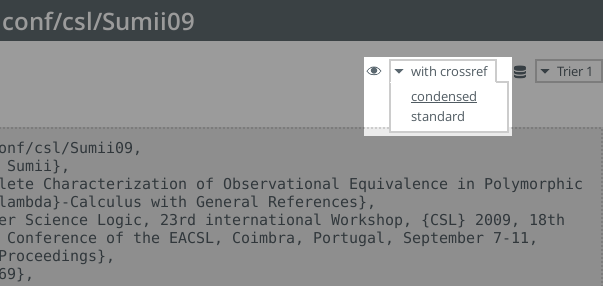
\includegraphics[width=.98\linewidth]{../docs/dblp_bibtex_crossref.png}
% \caption{試しに貼り付けられたdblp\_bibtex\_crossref}
% \label{f:aaa}
% \end{figure}

\chapter{提案手法}

\section{EbUをOCamlで実装するときの問題点}
Haskell版のEmbedding by Unembedding(EbU)ではHaskellの高度な機能である型クラス、GADT、型族、高階多相が用いられる。
しかし、OCamlでは型クラス、型族、高階多相の機能は存在しない。
特にEbUの実装に直接かかわる機能として、型族と高階多相があげられる。\\
 型族は型レベルの関数を表現する。
例えば、型レベルのリストの結合を定義したい場合、Haskellではソースコード\ref{src:haskell_append}のように定義する。
結合したいリストに対して、再帰的に{\tt Append}が適用され、リスト{\tt as}と{\tt bs}が結合されていることを確認できる。
この型レベルのリストの結合をOCamlでは直接実装することができない。\\
 高階多相は型オペレータを抽象化できることであり、ソースコード\ref{src:haskell_liftCore}で導入されている{\tt lift}の定義に用いられている。
OCamlには高階多相を直接表現する機能が存在しないため、Haskell版EbUの{\tt lift}関数に対応する関数を表現することが難しい。\\
% {\tt FuncSem}の{\tt sem}は高階多相であり、Haskellでは{\tt sem}の型から{\tt FuncSem}全体の型情報を推論することが可能である。
% しかし、OCamlでは高階多相が表現できないため、{\tt sem}の型を推論できず、結果的に全体の型を推論することができない。
%  高階多相はGADTを再帰的に定義するときに有利に働く。
% 例えば、\ref{src:haskell_liftCoren}の{\tt lift}関数を考える。
% {\tt lift}関数では{\tt h}について、{\tt h :: forall env. Env (SemRep sem env) ss $\rightarrow$ sem env r}と型を定義している。
% {\tt SemRep}はHaskellと同様、GADTで定義することになるが、OCamlではGADTの再帰的な定義をすることができない。
% 理由としては型推論時に型情報を失うからだ。\\
%  型クラスも同様である。
% Haskellではデータ型を定義する際に、その引数のデータ型に対して、明示的にカインドを書くことができる。
% 反対に、OCamlではカインドという概念がないため、カインドをプログラマが書くことができない。
% OCamlはGADTや型注釈により、カインドを記述できないながらも、ある程度の表現が可能である。
% しかし、複雑な型になると、型変数から型パラメータが推測できず、型の情報が失われる場合がある。\\
 以上のように、Haskellの高度な機能をOCamlで記述できないことがある。
このような高度な機能は別のデータ型を定義して回避したり、モジュールやファンクタを利用して書き換えたりすることで表現を行う。
Haskell版と同様に記述できる個所については、そのまま実装を行う。

\section{OCamlによるEbU}
3.2節ではOCaml版のEmbedding by Unembedding(EbU)の使用例を示す。EbUの使用に関しては2.3節の手順に従って行う。
例として、単純型付きラムダ計算(STLC)を扱う。\\
 ステップ1として、実装する言語の意味領域を特定する。
STLCの意味領域は、値環境を受け取り結果を返す。
% これは、値環境から結果までの関数を{\tt type}として定義
Haskell版と同様に以下のOCamlの型として定義することで、OCamlのデータ型として実装する。
STLCの意味領域の定義を以下に示す。

\begin{lstlisting}[%caption=意味領域の定義,label=src:semantic_domain
  ]
module VEnv = HList(struct type 'a t = 'a end)
type ('a, 'e) stlc = { runSim : 'e VEnv.hlist -> 'a }
\end{lstlisting}

% runSimはまさにSTLCのセマンティクスで、値環境から結果まで関数を表している。
環境はファンクタにより定義されており、異種混合リスト\cite{heterogeneous_oleg}を採用している。
異種混合リストにより、異なる型の値であっても、一つの環境で扱うことができる。
% この異種混合リストはまさにde Bruijn表現であるが、ユーザ側から直接扱うことはない。
以下のソースコードは異種混合リストの実装となる。

\begin{lstlisting}[%caption=異種混合リストの実装,label=src:hlist
  ]
module type HLIST = sig 
  type 'a el

  type _ hlist = 
    | HNil : unit hlist 
    | HCons : 'a el * 'r hlist -> ('a * 'r) hlist
end 

module HList (E: sig type 'a t end) 
      : HLIST with type 'a el = 'a E.t = struct ()
  type 'a el = 'a E.t 

  type _ hlist = 
    | HNil : unit hlist 
    | HCons : 'a el * 'r hlist -> ('a * 'r) hlist 
end
\end{lstlisting}

{\tt VEnv}を定義することで変数の型付け規則の解釈である{\tt var}と{\tt weaken}を実装できる。
% varの場合、runSimはVEnvから最初の要素を取り出す操作を行う。
% weakenの場合、VEnvの最初の要素を無視して新しいSimを構築する操作を行う。
Haskellでは{\tt var}と{\tt weaken}を{\tt Variables}型クラスとして定義したが、OCamlではファンクタにより定義する。
% {\tt var}や{\tt weaken}は{\tt Variables}型クラスとしてファンクタによりカプセル化される。
OCamlでは、ファンクタ{\tt Variables}を定義する前に、モジュール型{\tt VARIABLES}を定義する必要がある。
モジュール型{\tt VARIABLES}と、STLCにおけるファンクタ{\tt Variables}の定義を以下に示す。

\begin{lstlisting}[%caption=モジュール型VARIABLESの定義,label=src:Variables
  ]
module type VARIABLES = sig
  type (_, _) sem

  val var   : ('a, 'a * _) sem  

  val weaken : ('a , 'r) sem -> ('a , _ * 'r) sem
end

module VarSTLC = Variables (
  struct 
    type ('a, 'b) sem = ('a, 'b) stlc 

    let var = { runSim = function VEnv.HCons (x, _) -> x }
    
    let weaken = fun stlc -> 
      { runSim = function VEnv.HCons (_, venv') -> 
                                       stlc.runSim venv' }
end )
\end{lstlisting}

ステップ2として、言語要素の意味関数を定義する。
STLCには{\tt app}と{\tt lam}の二つの言語要素が存在する。\\
%  appは1次抽象構文の意味関数であり、STLC型に対する関数となる。
% appは関数適用であるため、関数fとその引数xの二つの引数を持ち、この二つの引数はSTLC型でラップされている。
% appの定義ではxにfが適用されるが、適用前にそれぞれの引数をrunSimによりアンパックする必要がある。\\
%  lamは2次抽象構文の意味関数であり、appと比較して複雑な言語要素となる。
% STLCでは、lamは環境内に引数がある場合に、STLC項を受け取り関数項を生成する。
意味関数の定義を以下に示す。

\begin{lstlisting}[%caption=意味関数の定義,label=src:semstlc
  ]
module SemSTLC = struct
  open STLC
  
  let appSem = fun fTerm aTerm ->
    { runSim = fun venv -> 
      let f = fTerm.runSim venv in
      let x = aTerm.runSim venv in
      f x }
  
  let lamSem = fun bTerm ->
    { runSim = fun venv x ->
      let g' = VEnv.HCons (x, venv) in 
      bTerm.runSim g' }    
end
\end{lstlisting}

% lamの関数項は、その引数を値環境に保存して、元の項を使用して結果を生成する。\\
step3では、埋め込む言語の構文のHOAS表現を提供する。
% step2で定義した意味関数は、ユーザにとっては使いやすいものではない。
% そのため、ユーザの扱いやすいHOAS表現でappやlamを表現する。
HOASでのSTLCの構文の提供を以下に示す。

\begin{lstlisting}[%caption=STLCのHOAS表現,label=src:hstlc
  ]
module type HSTLC = sig
  type 'a expr 

  val app : ('a -> 'b) expr -> 'a expr -> 'b expr
  val lam : ('a expr -> 'b expr) -> ('a -> 'b) expr
end
\end{lstlisting}

step4では、STLCの意味関数をHOASの構文に変換する意味モジュールを定義する。
意味モジュールの定義では、言語要素がどのような引数を持つかをargSpecに記述する。
argSpecはソースコード\ref{src:haskell_lift}の{\tt (LZ :. LZ :. End)}や{\tt ((LS LZ) :. End)}に対応する。
% この接続には、リフティング関数を提供している。
% lift関数で意味関数をラップして、toFunc関数に適用することで、適切に接続ができる。
% toFucnU関数はラップされた意味関数に、どのような引数を渡すかを決定している。
{\tt app}は引数の数が二つであり、一階の言語要素であるため、{\tt argSpec = XCons(XZ, XCons(XZ, XNil))}とする。
{\tt lam}は引数の数が一つであり、二階の言語要素であるため、{\tt argSpec = XCons(XS XZ, XNil)}となる。
% SConsが引数の数を表しており、Sはその引数にどのくらいの引数を含めるかを表している。
% toF関数のおかげで、1次抽象構文と2次抽象構文どちらにも同じリフティング関数を適用することが可能となった。
% そのため、ユーザは純粋にセマンティクスを考えるだけでよい。
{\tt lift}関数による意味モジュールの定義を以下に示す。

\begin{lstlisting}[caption=意味モジュールの定義,label=src:lifting_fun]
module STLC_sem : HSTLC with type 'a expr = 'a STLC.VarSTLC.envi = 
  struct 
    type 'a expr = 'a VarSTLC.envi
    open STLC open VarSTLC 
  
    let app : 
      type a b. (a -> b) envi -> a envi -> b envi = fun e1 e2 -> 
      let argSpec = XCons (XZ, XCons (XZ, XNil)) in
        toF argSpec 
          (liftCore' {f = fun x -> fromF argSpec SemSTLC.appSem x}) 
          e1 e2
  
    let lam : 
      type a b. (a envi -> b envi) -> (a -> b) envi = fun e ->
      let argSpec = XCons (XS XZ, XNil) in 
        toF argSpec 
          (liftCore' {f = fun x -> fromF argSpec SemSTLC.lamSem x}) 
          e  

    let runOpenSTLC : 
      type a b.(a expr -> b expr) -> (b, a * unit) stlc = fun f ->
        VarSTLC.runOpen f 
  end 
\end{lstlisting}

% 内部では環境をde Bruijnインデックスで管理をしている。しかし、このde Bruijnインデックスの型とユーザが扱うHOAS表現の型の間で型の不一致がある。
% そのため、型をラップして、この型の不一致を解消する。型のラップはenviで定義されており、それを\ref{src:envi}に示す。

% \begin{lstlisting}[caption=EnvIの定義,label=src:envi]
% type 'a envi = { runEnvI : 'e. 'e TEnv.hlist -> ('a, 'e) sem}
% \end{lstlisting}

ステップ5では、実際に言語を機能させる。
EbUは{\tt Variables}型クラスの意味に対して一般的に開いた式の解釈を提供しており、OCaml版でも同様に提供している。
その解釈を以下に示す。

\begin{lstlisting}[%caption=開いた式の解釈,label=src:runopen
  ]
let runOpen : type a b. (a envi -> b envi) -> 
                                    (b, a * _) sem = fun f -> 
  let eA = TEnv.HCons ((), TEnv.HNil) in 
  let x  = { runEnvI = fun e' -> weakenMany eA e' H.var} in 
  (f x).runEnvI eA 
\end{lstlisting}

自由変数が一つであるケースには、{\tt runOpen}は開いた式を受け取り、意味領域に変換する。
自由変数が一つであることを確認するには、{\tt runOpenSTLC}でラップする必要がある。
以下に{\tt runOpenSTLC}を示す。

\begin{lstlisting}[%caption=runOpenのラップ,label=src:runopenstlc
  ]
module type OPEN_STLC_TERM = sig 
  type in_t 
  type out_t 

  module OpenTerm(L : HSTLC) : sig val res : in_t L.expr -> 
                                             out_t L.expr end 
end 

type ('a, 'b) open_stlc_term = 
  (module (OPEN_STLC_TERM with type in_t = 'a and type out_t = 'b))

let runOpenSTLC : type a b. 
  (a, b) open_stlc_term -> (b, a * unit) stlc = 
    fun (module OT) -> 
      let module M = OT.OpenTerm(STLC_sem) in 
      STLC_sem.runOpenSTLC M.res
\end{lstlisting}

ここまでで、一般的な開いた式に対する実行関数を定義したため、次にSTLCを動作させる関数を定義する。
STLCを動作には、以下の関数を利用する。

\begin{lstlisting}[%caption=開いた式の解釈,label=src:runstlc
  ]
let runSTLC = fun t x ->
  let g = VEnv.HCons (x, VEnv.HNil) in 
  t.runSim g
\end{lstlisting}

この関数は自由変数が一つのSTLC項に対して動作する。
実際に、値3を持つ自由変数への恒等関数の適用を評価する。
すると、以下のソースコードの実行に対して、次のような結果が得られる。

\begin{lstlisting}[%caption=実行例,label=src:ex
  ]
module TM = struct 
  type in_t = int type out_t = int
  module OpenTerm(L : HSTLC) = struct 
    open L 
    let res x = app (lam (fun y -> y)) x 
  end 
end

let ex = fun x -> 
  STLC_sem.runSTLC (STLC.runOpenSTLC (module TM)) x 

ex 3
\end{lstlisting}

{\tt val ex : 'a STLC.STLC\_sem.expr $\rightarrow$ 'a STLC.STLC\_sem.expr = <fun>\\ val ex : int = 3 }

\section{liftCoreの実装}
% EbUはlift関数により、構文とセマンティックを接続している。
% lift関数はEbUにおいて重要な関数であるが、実装は複雑になる。
% 複雑になる理由として、意味関数の各引数が任意の数の引数をバインドするためである。
% バインドする引数の数が異なるため、それぞれの引数に対して異なる処理をする必要がある。\\
{\tt lift}関数はHaskellの高度な機能を使い実装されている。
OCamlで実装はstraightforwardではないが、Haskell版のEbUと同様の手順で実装する。
 はじめに、{\tt sig2}データ型を用意する。
{\tt sig2}の定義は以下のように示す。
% sig2型は言語要素の引数に対して型付けをしており、これにより埋め込みされていない解釈の型の定義が可能となる。

\begin{lstlisting}[%caption=sig2の定義,label=src:sig2
  ]
type ('xs, 'x) sig2 = |
\end{lstlisting}

続いて、{\tt HoasRep}と{\tt SemRep}のデータ型を定義する。この定義を以下に示す。\\

\begin{lstlisting}[%caption=HoasRepとSemRepの定義,label=src:HoasRep_SemRep
  ]
type (_,_) SemRep = 
  | TR : ('xs,'env,'r) wapp * ('x, 'r) sem -> 
                    ('env, ('xs, 'x) sig2) SemRep

type (_) HoasRep =
  | UR : 'xs TEnv.hlist * ('xs HListEnvI.hlist -> 'x envi) -> 
                                            ('xs,'x) sig2 HoasRep 
\end{lstlisting}

% HoasRepは言語要素の各引数の型情報のリストであり、引数の型環境xsの値レベルの表現をとる。
% これにより、各引数の型付け情報を得られる。\\
%  SemRepは入力された2次抽象関数の項の型付け規則を表している。
% 2次抽象関数の型付け規則は以下のようになる。

% \begin{prooftree}
%   \AxiomC{$\Gamma,~x:\alpha \vdash e:\beta$}
%   \UnaryInfC{$\Gamma \vdash \lambda x.~e:\alpha \rightarrow \beta$}
% \end{prooftree}

% 入力された項を型付けする場合、もちろん型付け環境が必要となる。
% しかし、もともとのセマンティクスには$\Gamma$と$\alpha$をAppendした環境が含まれている。
% そのため、型付け環境$\Gamma$を得るため、SemRepは必要となる。\\
ここで、ソースコード\ref{src:haskell_uSemRep}に注目する。
{\tt SemRep}の定義には、型環境の対する{\tt Append}が含まれており、この{\tt Append}は型族を用いて定義されている。
しかし、OCamlでは型族を表すことができない。
そのため、Haskellの{\tt Append}に該当する操作として、新しく{\tt wapp}を定義する。
{\tt wapp}の定義を以下に示す。

\begin{lstlisting}[%caption=wappの定義,label=src:wapp
  ]
type (_,_,_) wapp =
  | AppNil  : (unit, 'b, 'b) wapp
  | AppStep : ('x , 'y , 'r) wapp -> ('a * 'x, 'y, 'a * 'r) wapp
\end{lstlisting}

{\tt wapp}は型レベルのリストが入れ子の組で表現されている。
{\tt wapp}は三つ型パラメータを持ち、その関係は{\tt ('x, 'y, 'r) wapp}に対して \\
$'r~=~'x~++~'y$ となる。
これにより、疑似的に{\tt Append}を表現でき、OCamlで直接表現できない型の表現を回避できる。\\
 以上により、{\tt liftCore}関数の実装の準備ができた。以下に{\tt liftCore}関数の実装を示す。

\begin{lstlisting}[%caption=liftCoreの実装,label=src:liftCore
  ]
let liftCore : 
  type ss rr. (ss,rr) semTerm -> ss HoasRepEnv.hlist -> rr envi = 
    fun ff ks -> 
    { runEnvI = fun (type env) (e : env TEnv.hlist) -> 
      let module App = HListP(TEnv) in
      let module M_map = MapToSemRepHList(HoasRepEnv) in  
      let rec mkXs : type env ys ys_env. env TEnv.hlist
          -> ys TEnv.hlist
          -> (ys, env, ys_env) wapp 
          -> ys_env TEnv.hlist -> ys HListEnvI.hlist =
           fun p ys wit te -> 
           match ys, wit, te with
           | HNil, _, _ -> HNil 
           | (HCons(_,ys')),AppStep(wit'),HCons(_,te') ->
             let x = { runEnvI = fun e' -> weakenMany te e' H.var} 
              in HCons(x,mkXs p ys' wit' te') 
          in                       
      let cnv : type env xs x. env TEnv.hlist -> xs TEnv.hlist 
                 -> (xs HListEnvI.hlist -> x envi)
                 -> (env, (xs,x) sig2) SemRep = fun e e1 k -> 
         match App.append_hlist e1 e with
         | AppHList(wit, ex_e) -> 
           let xs = mkXs e e1 wit ex_e in 
           TR(wit, (k xs).runEnvI ex_e) in 
      let conv : type env s. env TEnv.hlist -> s HoasRep -> 
                                            (env,s) SemRep =
       fun e ur -> match ur with 
       | UR(e1, k) -> cnv e e1 k in      
      ff.f (M_map.map {f = fun xs -> conv e xs} ks)
    }
\end{lstlisting} 

{\tt liftCore}関数の型に注目する。
Haskell版の{\tt liftCore}関数の型は{\tt (forall env. Env (SemRep sem env) ss $\rightarrow$ sem env r) $\rightarrow$ Env (HoasRep sem) ss $\rightarrow$ EnvI sem r}となっているが、
OCaml版の型では{\tt (ss,rr) semTerm $\rightarrow$ ss HoasRepEnv.hlist $\rightarrow$ rr envi}となっており、第一引数の型が一見異なるように見える。
これはOCamlでは高ランク多相を直接表現できないためであり、代わりにフィールドに多相型のレコードを用意する。
{\tt semTerm}の定義を以下に示す。

\begin{lstlisting}[%caption=semTermの定義,label=src:semTerm
  ]
type ('ss,'rr) semTerm = {f: 'env. ('env,'ss) SemRepEnv_hlist -> 
                                                  ('rr, 'env) sem }
\end{lstlisting}

{\tt SemRepEnv\_hlist}はHaskell版における{\tt Env (SemRep sem env) ss}に対応しており、以下のように定義される。

\begin{lstlisting}[%caption=SemRepEnv_hlistの定義,label=src:semrephlist
  ]
type ('env,_) SemRepEnv_hlist =
  | THNil  : ('env,unit) SemRepEnv_hlist
  | THCons : ('env,'s) SemRep * ('env, 'ss) SemRepEnv_hlist 
                            -> ('env,'s * 'ss) SemRepEnv_hlist
\end{lstlisting}

Haskell版の定義では{\tt Env (SemRep sem env) ss}は高階多相を利用して定義されているが、3.1節でも述べた通りOCamlには高階多相を直接表現する手段がない。
そのため、GADTを利用することで、高階多相が必要になることを回避した。
以上を踏まえ、{\tt semTerm}の定義を見ると、{\tt (forall env. Env (SemRep sem env) ss $\rightarrow$ sem env r)}を表せることが確認できる。\\

% \begin{lstlisting}[caption=toFの定義,label=src:haskell_toF]
% toF :: Dim ss -> (Env (HoasRep sem) ss -> EnvI sem r) -> FuncU sem ss r
% fromF :: FuncSem sem env ss r -> Env (SemRep sem env) ss -> sem env 
% \end{lstlisting}

\section{利便性の高いAPIの提供}
HOASの構文と意味関数の変換を行う関数は{\tt liftCore}関数であるが、Haskell版の{\tt lift}関数を見ると、{\tt toF}や{\tt fromF}といった、補助関数が見受けられる。
これらの関数はユーザの利便性を向上させるために導入された関数である。
そのため、本節でもユーザビリティのため、{\tt toF}や{\tt fromF}を実装する。\\
 はじめに、{\tt toF}関数を定義する。
{\tt toF}関数は環境に追加された型情報をHOASに変換する関数である。
しかし、関数の内容自体は複雑ではなく、アンカリー化をするような動作を行う。
そこであらかじめ、アンカリー化を行うファンクタを以下に定義する。

% \begin{lstlisting}[caption=toFの定義,label=src:haskell_toF]
% toF :: Dim ss -> (Env (HoasRep sem) ss -> EnvI sem r) -> FuncU sem ss r
% fromF :: FuncSem sem env ss r -> Env (SemRep sem env) ss -> sem env 
% \end{lstlisting}
\begin{lstlisting}[%caption=uncurryの定義,label=src:lift_uncurry
  ]
module CurryUncurry(H : HLIST) = struct
  type (_,_,_) cspec = 
    | Z : ('r, 'r, unit) cspec 
    | S : ('r, 'f, 'xs) cspec -> 
          ('r, 'a H.el -> 'f, ('a * 'xs)) cspec 

  let rec uncurry : 
    type r f xs. (r,f,xs) cspec -> f -> xs H.hlist -> r = 
    fun s h args -> match s, args with  
    | Z ,   _           -> h 
    | S ss, HCons(x,xs) -> uncurry ss (h x) xs   

  let rec cspec2TEnv : 
    type r f xs. (r, f, xs) cspec -> xs TEnv.hlist = 
      fun n -> match n with   
      | Z -> TEnv.HNil 
      | S s' -> TEnv.HCons ((), cspec2TEnv s')
end
\end{lstlisting}

{\tt cspec}型は{\tt uncurry}を行う回数を表すデータ型である。
{\tt cspec2TEnv}は{\tt cspec}と同じ大きさの型リストを作成する関数である。
続いて、{\tt toF}の型を考える。
ソースコード\ref{src:haskell_toF}を見ると、{\tt toF}関数の定義に型族が用いられている。
OCamlでは型族を直接表現できないため、{\tt FuncU}に対応するGADTを以下にに定義する。

\begin{lstlisting}[%caption=tf\_specの定義,label=src:lift_tf_spec
  ]
type (_,_,_) tf_spec =
  | SNil  : ('rr, 'rr, unit) tf_spec 
  | SCons : ('x envi, 'f, 'xs) cspec * ('rr, 'ff, 'ss) tf_spec -> 
            ('rr, 'f -> 'ff, (('xs, 'x) sig2 * 'ss)) tf_spec 
\end{lstlisting}

{\tt tf\_spec}は{\tt FuncU}のほかに、{\tt Dim}にも対応している。
これにより、{\tt toF}関数の定義の準備ができた。
{\tt toF}関数の定義を以下のように示す。

\begin{lstlisting}[%caption=toFの定義,label=src:ocaml_toF
  ]
let toHoasRep : type f xs x. (x envi, f, xs) cspec -> 
  f -> (xs,x) sig2 HoasRep
    = fun cs f -> UR (cspec2TEnv cs, uncurry cs f)

let rec toF : type rr ff ss. (rr envi,ff,ss) tf_spec -> 
  (ss HoasRepEnv.hlist -> rr envi) -> ff
    = fun tfs h -> match tfs with
      | SNil -> h HNil 
      | SCons(cs,tfs) -> fun k -> 
        toF tfs (fun r -> h (HCons(toHoasRep cs k,r)))
\end{lstlisting}

続いて、{\tt fromF}の定義を行う。
{\tt fromF}関数は型付け環境に新しく追加された型付け規則を集める関数である。
{\tt fromF}関数の実装は{\tt toF}関数の実装方法と同じである。
{\tt fromF}関数も{\tt toF}関数と同様にアンカリー化をする関数であるが、型付け規則を収集するため、それに対応する新しいGADT{\tt FuncSem}を導入する必要がある。
以下にに{\tt FuncSem}に対応するGADTを示す。

\begin{lstlisting}[%caption=ff\_specの定義,label=src:lift_ff_spec
  ]
type (_,_,_,_,_) ff_spec = 
  | FNil  : ('dummy, 'env,'rr, ('rr,'env) sem,unit) ff_spec 
  | FCons : ('xs,'env,'app) wapp  * 
            ('dummy,'env,'rr,'ff,'ss) ff_spec -> 
            ('app * 'dummy, 'env, 'rr, ('x,'app) sem -> 
              'ff , (('xs,'x) sig2 * 'ss)) ff_spec
\end{lstlisting}

{\tt ff\_spec}には{\tt dummy}型が含まれる。この{\tt dummy}型は{\tt app}型を保存するために利用される。
本来、{\tt app}型は型推論により型を決定されるが、OCamlでは{\tt app}型の型推論を行うことができない。
そのため、意図的に{\tt dummy}型を導入して、{\tt app}型の型を推論できるようにする。\\
 {\tt ff\_spec}により{\tt fromF}関数が定義できる。
以下にに{\tt fromF}関数を定義する。

\begin{lstlisting}[%caption=fromFの定義,label=src:ocaml_fromfunc
  ]
let rec fromF : 
  type dummy env res tt ss. 
    (dummy, env, res, tt, ss) ff_spec -> tt -> 
    ((env, ss) SemRepEnv_hlist -> (res,env) sem) = 
      function 
      | FNil -> fun x _ -> x 
      | FCons (w1, fs) -> fun f -> function 
        | THCons(TR(w2,t),ts) -> match wapp_functional w1 w2 with 
          | Refl -> fromFunc fs (f t) ts
\end{lstlisting}

{\tt toF}関数と同様、型族の実装以外は{\tt fromF}関数の定義と異なる点はない。\\
 以上により、{\tt lift}関数の定義の準備が整った。
{\tt lift}関数の利用方法はソースコード\ref{src:lifting_fun}に示すとおりである。
{\tt toF}関数と{\tt fromF}関数で扱うGADTは型は異なるが、形は同じになる。
EbUの利便性のため、{\tt toF}関数と{\tt fromF}関数で扱うGADTはまとめて定義したい。
そこで、新しいGADTとして以下のGADTを定義する。

\begin{lstlisting}[caption=arg\_specの定義,label=src:lift_arg_spec]
type (_,_,_,_,_,_) arg_spec =
  | XNil  : ('dummy, 'env, 'rr, 'rr envi, 
             ('rr,'env) sem, unit) arg_spec 
  | XCons : 
      ('xs, 'env, 'app, 'x envi, 'f) wapp_cspec * 
      ('dummy, 'env, 'rr, 'toFunc, 'fromFunc, 'ss) arg_spec -> 
      ('app * 'dummy, 'env, 'rr, 'f -> 'toFunc, ('x,'app) sem -> 
                    'fromFunc, (('xs,'x) sig2 * 'ss)) arg_spec
\end{lstlisting}

このGADTにより、ユーザが記述する言語要素の引数の情報は一つだけでよくなる。
ソースコード\ref{src:lifting_fun}で利用される{\tt toF}や{\tt fromF}は、{\tt arg\_spec}を{\tt tf\_spec}や{\tt ff\_spec}に変換し、{\tt toF}関数や{\tt fromF}関数に適用する関数である。

以上より、OCaml版EbUのlift関数を定義できる。
しかし、OCaml版EbUとHaskell版EbUのlift関数の記述方法を比較すると少々相違点が見受けられる。
Haskell版のEbUの{\tt lift}関数は言語要素の引数の情報と意味関数を引数として与えるだけで、HOASと意味関数の変換を行える。
一方で、OCaml版のEbUの{\tt lift}関数は{\tt argSpec}で言語要素の各引数の束縛の情報を表現し、{\tt toF}、{\tt fromF}、{\tt liftCore}、{\tt argSpec}の4つの関数を利用することで意味モジュールの定義を行う。
OCaml版のEbUは、本来言語実装者に見せたくない{\tt toF}や{\tt fromF}、{\tt liftCore}を明示的に与えている。
% これは、OCamlでは高ランク多相をフィールドやファンクタでしか表現できないことに起因する。
% {\tt argSpec}はGADTで定義されており、再帰的に定義をすることが難しい。
この原因も3.1節で述べたOCamlが高階多相を直接表現する機能がないことに起因する。
実際に、以下の素朴な{\tt lift}関数の実装は型整合ではない。

\begin{lstlisting}[%caption=OCamlで定義できないlift関数,label=src:ocaml_lift_false
  ]
let lift = fun e argSpec sem -> 
  toF argSpec (liftCore' {f = fun x -> fromF argSpec sem x}) e
\end{lstlisting}

仮にOCamlに高階型変数を表現する機能が存在すれば、Haskell版の{\tt lift}関数の型
{\tt forall sem ss r. Variables sem => Dim ss -> (forall env. FuncSem sem env ss r) -> FuncU sem ss r}
を、簡便のため一階の高ランク多相を許したとして
{\tt {'env. (...,'env,'r,'t,'env,'f,'ss) arg\_spec} -> {'env. 'env 'f} -> 't}
と書ける。
しかし、'fが高階の型変数であるためこのような型はOCamlで表現可能ではない。
% として定義できるが、OCamlでは{\tt t}が{\tt 'env f}の形になっていることを直接表現できない。
ファンクタを用いることで同等の型が表現できることが予想されるが、素朴にはソースコード\ref{src:lift_arg_spec}でいうところの'xや'xsを陽に渡す必要が生じ、ユーザビリティを大きく損う。\\
% 束縛の表現を陽に{\tt lift}関数に渡す必要があり、ユーザビリティを大きく損う。\\
% したがって、OCamlの機能のみでは現状Haskell版EbUの{\tt lift}関数を定義できない。\\
 この問題を解決するためにppxを利用することを検討している。
ppxはOCamlで利用できるプリプロセッサである。
ppxにより、{\tt toF}、{\tt fromF}、{\tt liftCore}を隠蔽し、Haskell版の{\tt lift}関数に対応する関数をOCamlで提供することが可能となる。
{\tt lift}関数をOCamlで提供できれば、ユーザビリティの高いAPIをEbUユーザに提供可能できる。\\
もしくは、5章で述べるYallopとWhiteの手法\cite{hkp_yallop}を利用することでfunctorに頼らない実装が可能になると考えれらる。
これに関して詳しくは、5.2節にて述べる。
% そのため、ユーザの負担を軽減するためにAPIを提供する。
% このAPIはHaskell版のEbUをもとに、型族や型クラスを回避して実装を行う。
% ユーザは\ref{src:lifting_fun}からわかる通り、
% $(toF~(SCons~...~) (liftCore~\{~f~=~fun~x \rightarrow fcons~...~sem~x~\}))$
% として、リフティング関数を実行可能である。
% toF関数とliftCore関数を利用して、言語要素の各引数によってバインディングされる変数の数(SCons)と、各引数が型環境に対してどの回数Appendの操作を行うか(fcons)を指定するだけでよい。
% ただし、SConsとfconsは明らかに等しい回数になるため、ユーザは片方の定義が完了したら、もう一方の定義は機械的に定義できる。\\
%  Haskell版のEbUは型族によって、FuncUというデータ型を定義して、セマンティクスを定義する。
% しかし、OCamlではFuncUは定義できないため、toF関数から直接セマンティクスを定義する。
% \ref{src:toF}にtoF関数を示す。

% \begin{lstlisting}[caption=toF関数の実装,label=src:toF]
% let rec toF : 
%      type rr ff ss. 
%      (rr envi,ff,ss) tf_spec -> 
%                       (ss HoasRepEnv.hlist -> rr envi) -> ff
%       = fun tfs h -> match tfs with
%         | SNil -> h HNil 
%         | SCons(cs,tfs) -> fun k -> 
%             toF tfs (fun r -> h (HCons(toHoasRep cs k,r)))  
% \end{lstlisting}

% toF関数の最終的な型はffであるが、ffはenviデータ型を示しているため、toF関数はセマンティクスを定義することを確認できる。
% toHoasRepは言語要素の各引数からHoasRepデータ型を生成する関数である。
% $(HCons(toHoasRep~cs~k,~r))$はHoasRepEnvを表現していることから、実際にはtoF関数はHoasRepEnvを生成してliftCore関数に適用している関数となる。\\
%  toF関数とliftCore関数の実装の形態は決まっているため、SConsと意味関数が定義できれば、リフティング可能である。
% 現在はtoFをユーザが利用するが、最終的にはtoF関数とliftCore関数を組み合わせたliftCoren関数を実装を考えている。
% ユーザは一つの関数しか利用する必要がないため、さらに利便性が向上すると予想される。



\chapter{評価}
\section{EDSLの実装方法}
3章で定義したEmbedding by Unembedding(EbU)を用いて、増分計算(ILC)\cite{ilc2014_Cai}の埋め込みを行う。
ILCはユーザ入力された計算と、その差分の計算を同時に行う計算体系である。
例として、入力された自然数に対して2乗を行う式を考える。
ユーザが 

$f~x~=~x^2$

と入力すると、システム内部ではユーザ入力に対する差分として、

$df~x~dx~=~2~*~x~*~dx~+~dx~*~dx$

を計算する。\\
 結果を得るには入力した式に対して、具体的な値を代入すればよい。
例えば、通常の結果を得たいとき、ユーザの入力$f~5$に対して、25を出力する。
差分の結果が得たいとき、$x~=~5$に対して、その差分2の結果は$df~5~2$を入力すると、24が得られる。
これは$f~(5~+~2)~-~f~5$の結果と一致する。\\
 ILCの意味領域は一般的に以下のようになる。

$A \rightarrow B,~A \rightarrow \Delta A \rightarrow \Delta B$

Aは入力、$\Delta A$は入力の差分、Bは出力、$\Delta B$は出力の差分を表す。
つまり、ILCは以下の二つの意味領域を持つ。

\begin{itemize}
  \item 通常の評価を行い、入力に対して結果を出力する
  \item 差分の評価を行い、入力と入力の差分に対して結果の差分を出力する
\end{itemize}

この意味領域を、二つのアイディアによって定義する。\\
 一つ目は対象言語の項に対する型付けを$e~:~A$から$e~:~<A,~\Delta A>$に拡張して、Aと$\Delta A$の両方行うことである。
これは、あくまで型付けを二つ行うことであり、組として扱うわけではない。\\
 二つ目は、$e~:~<A,~\Delta A>$を組として表現して、

$[(A_1,\Delta A_1),...,(A_n,\Delta A_n)]~H.hlist \simeq A_1*...*A_n*unit$

として、型付け環境を表すことである。{\tt hlist}とすることで、型環境の表現を容易に行うことができる。
ただし、この表現方法のみだとmapやconcat等の実装が困難になる。
一般にはAと$\Delta A$のだけではなく、項の変更を反映するための関数も保持する必要がある。
この問題はEbUの問題ではなく、ILCの複雑さに起因するものである。
そのため、本研究ではこの問題を扱わず、項を反映するための関数の保持が必要のないケースについてのみ議論する。\\
 以上のことをふまえ、意味領域は以下のようになる。

\begin{lstlisting}[%caption=ILCの意味領域,label=src:ilc_semantic_domain
  ]
type ('x, 'xs) ilc = 
    ('xs H.hlist -> 'x FromFst.t) 
  * ('xs H.hlist -> 'xs D.hlist -> 'x FromSnd.t)             
\end{lstlisting}

これは$\Gamma \vdash e~:~A$の意味領域$(\llbracket \Gamma \rrbracket \rightarrow \llbracket A \rrbracket) \times (\llbracket \Gamma \rrbracket \rightarrow \Delta \llbracket \Gamma \rrbracket \rightarrow \Delta \llbracket A \rrbracket)$に対応する。
{\tt FromFst}や{\tt FromSnd}はILCの出力であるBや$\Delta B$を表すモジュールである。\\
 意味領域を定義できたため、残りの埋め込みに関しては3章2のとおりに行う。
まず、ILCの意味関数は加算を行う{\tt addSem}、乗算を行う{\tt mulSem}、組の第一要素を取る{\tt fstSem}、組の第一要素を取る{\tt sndSem}、変数を束縛する{\tt letSem}を定義する。
% なお、fstSemとsndSemの式はほぼ同じになるため、sndSemは省略する。
以下ににILCの意味関数の定義を示す。

\begin{lstlisting}[%caption=ILCの意味関数,label=src:ilc_sem_fun
  ]
module SemILC = struct
open ILC

let addSem : type env. 
  (int * int, env) ilc -> (int * int, env) ilc -> 
  (int * int, env) ilc =
    fun (f, df) (g, dg) -> 
      (fun theta -> 
        let FFst v = f theta in 
        let FFst w = g theta in 
        FFst (v + w)) , 
      (fun theta dtheta -> 
        let FSnd dv = df theta dtheta in 
        let FSnd dw = dg theta dtheta in 
        FSnd (dv + dw))

let mulSem : type env. 
  (int * int, env) ilc -> (int * int, env) ilc -> 
  (int * int, env) ilc = 
    fun (f, df) (g, dg) -> 
      (fun theta -> 
        let FFst v = f theta in 
        let FFst w = g theta in 
        FFst (v * w)),
      (fun theta dtheta -> 
        let FFst v = f theta in 
        let FFst w = g theta in
        let FSnd dv = df theta dtheta in 
        let FSnd dw = dg theta dtheta in 
        FSnd (v * dw + dv * w + dv * dw) 
        )

let fstSem : type env a da b db. 
  ((a * b) * (da * db) , env) ilc -> (a * da, env) ilc = 
    fun (f, df) -> 
      (fun theta -> 
       let FFst (v, _) = f theta in 
           FFst v), 
      (fun theta dtheta -> 
       let FSnd (dv,_) = df theta dtheta in
           FSnd dv  
      )

let sndSem : type env a da b db. 
  ((a * b) * (da * db) , env) ilc -> (b * db, env) ilc = ...

let letSem : type env a b. 
  (a, env) ilc -> (b, (a * env)) ilc -> (b, env) ilc = 
    fun (f, df) (g, dg) -> 
      (fun theta -> 
       let FFst v = f theta in 
       let FFst w = g (HCons(FFst v,theta)) in 
           FFst w), 
      (fun theta dtheta -> 
       let FFst v = f theta in 
       let FSnd dv = df theta dtheta in 
           dg (HCons(FFst v, theta)) (HCons(FSnd dv,dtheta))
      )
end 
\end{lstlisting}

続いて、ILCのHOASを与える。
HOASは{\tt let\_}、{\tt add}、{\tt mul}、{\tt fst}、{\tt snd}の5つを定義する。
% addとmulのHOAS、fstとsndのHOASは形式が同じであるため、mulとsndのHOASは省略する。
ILCのHOASを以下に示す。

\begin{lstlisting}[%caption=ILCのHOASの構文,label=src:ilc_sem_hoas
  ]
module type HILC = sig 
  type 'a expr 

  val let_ : 'a expr -> ('a expr -> 'b expr) -> 'b expr 
  val add  : (int * int) expr -> (int * int) expr -> (int * int) expr 
  val mul  : (int * int) expr -> (int * int) expr -> (int * int) expr 
  val fst  : (('a * 'b) * ('da * 'db)) expr -> ('a * 'da) expr 
  val snd  : (('a * 'b) * ('da * 'db)) expr -> ('b * 'db) expr
end 
\end{lstlisting}

続いて、意味関数とHOASを接続する。
{\tt let\_}のみsecondの言語要素であるため、{\tt lift}関数に渡す引数の情報について注意する。
% また、addとmulのlift関数の内容、fstとsndのlift関数の内容が同じであるため、mulとsndのlift関数については省略する。
以下にに意味関数とHOASを接続するプログラムを示す。

\begin{lstlisting}[%caption=ILCの意味モジュールの定義,label=src:ilc_sem_hoas
  ]
module HILC_sem : HILC = struct 
  open ILC 
  type 'a expr = 'a VarILC.envi 
  open VarILC

  let let_ = fun e1 e2 -> 
    let argSpec = XCons (Z, XCons (S Z, XNil)) in
    toF argSpec 
    (liftCore' {f = fun x -> fromF argSpec SemILC.letSem x}) e1 e2
    e1 e2 

  let add = fun e1 e2 -> 
    let argSpec = XCons (Z, XCons (Z, XNil)) in 
    toF argSpec 
    (liftCore' {f = fun x -> fromF argSpec SemILC.addSem x}) e1 e2 

  let mul = fun e1 e2 -> 
    let argSpec = XCons (Z, XCons (Z, XNil)) in 
    toF argSpec 
    (liftCore' {f = fun x -> fromF argSpec SemILC.mulSem x}) e1 e2 

  let fst = fun e -> 
    let argSpec = XCons (Z, XNil) in 
    toF argSpec 
    (liftCore' {f = fun x -> fromF argSpec SemILC.fstSem x}) e 

  let snd = fun e -> 
    let argSpec = XCons (Z, XNil) in 
    toF argSpec 
    (liftCore' {f = fun x -> fromF argSpec SemILC.sndSem x}) e 
end
\end{lstlisting}

% 最後に、ILCを実行する。
これにより、ILCを埋め込むことができたため、あとはILCを実行すればよい。

\section{Haskell版との比較}
OCaml版のEbUとHaskell版のEbUで実装されたILCには比較すると大きく二つの相違点がある。\\
 一つ目は意味領域の定義方法である。
Haskell版ではILCの意味領域を以下のように定義している。

\begin{lstlisting}[caption=HaskellにおけるILCの意味領域,label=src:haskell_ilc_sem_dom]
data ILC env a = Inc
  { sEval :: VEnv env -> a, 
    dEval :: VEnv env -> DEnv env -> Delta a }
\end{lstlisting}

Haskell版のILCとOCaml版のILCでは意味領域の考え方は同じであるが、その定義方法が大きく異なる。
Haskell版では{\tt DEnv}の定義をopen type familyによって行う。
これにより、{\tt DEnv}の型を後から変更することができるため、項によらずに型環境を扱うことができる。
OCamlでは型族の代わりにGADTを用いて実装を行ったが、OCamlのGADTではあらかじめ型を記述する必要があるため、open type familyをGADTで表現できない。
そのため、OCamlではまず、通常の入力と差分の入力を表すモジュールを以下のように定義した。

\begin{lstlisting}[%caption=OCamlにおけるILCの意味領域の準備,label=src:ocaml_ilc_module
  ]
module FromFst = struct 
  type _ t = 
  | FFst : 'a -> ('a * 'd) t  
end 

module FromSnd = struct 
  type _ t = 
  | FSnd : 'd -> ('a * 'd) t  
end
\end{lstlisting}

次に、{\tt FromFst}や{\tt FromSnd}を要素とする{\tt hlist}を考え、{\tt DEnv}と同等の表現力を持たせた。
本研究で扱かったILCはこのような方法で意味領域を表現することができたが、扱う計算体系によっては意味領域をOCamlで表現しきれない可能性がある。
本論文ではOCaml版のEbUで埋め込むことができる計算体系の範囲は議論しないが、これは今後検討したい。\\
 二つ目は{\tt lift}関数の利用方法である。
ただし、この議論は3.4でも行ったため、省略する。\\
 以上の2点がOCaml版のEbUとHaskell版のEbUの相違点である。
ILC以外の高度な意味の意味領域の実装方法、
OCamlにおける高階多相のフィールドやファンクタを用いない表現方法が明らかになればOCaml版のEbUもHaskell版のEbUと同等のユーザビリティが得られると考えられる。

\chapter{関連研究}
\section{type\-indexed valueの表現}
% 本研究では、型族をGADTで実装したが、型族を関数として表現することも可能である。
本研究では、{\tt toF}や{\tt fromF}をGADT {\tt arg\_spec}を引数に取る関数として実装したが、
これらはYang\cite{YANG2004151}のtype-indexed valueの表現手法の一つを用いても実装可能でなる。
% 例えば、\ref{src:lift_ff_spec}の{\tt ff\_spec}の定義は{\tt dummy}を意図的に含めることで{\tt app}の推論を可能にした。
% しかし、{\tt dummy}を消すと{\tt app}の推論を行えず、{\tt ff\_spec}の実装ができない。
% これに対して、YangはML言語における型族の表現についてみつの方法を提供している\cite{YANG2004151}。
% その中で、Yangは型族を型に対応する値としてエンコードする方法を紹介する方法も紹介しているが、これにより{\tt ff\_spec}を関数で表現することができる。
type-indexed valueをGADTを用いて、{\tt f :: Sing a -> F a}のような形で値レベルの表現を表すGADTを引数に取ることで表せる。
% {\tt toF}や{\tt fromF}はまさにtype-indexed valueであるため、Yangの手法で表現ができる。
実際に{\tt fromF}で扱うGADT({\tt ff\_spec})を、Yangの手法で表すと以下のようになる。
% {\tt ff\_spec}を表現する関数を\ref{src:ocaml_ff_spec_fun}に示す。

\begin{lstlisting}[caption=ff\_specを表すtype-indexed value,label=src:ocaml_ff_spec_fun]
let fnil : ('r,'env) sem -> ('env,unit) SemRepEnv_hlist 
                         -> ('r,'env) sem = fun x _ -> x 
let fcons : 
  ('xs,'env,'app) wapp 
  -> ('ff -> ('env,'ss) SemRepEnv_hlist -> ('r,'env) sem)
  -> ((('x,'app) sem -> 'ff) 
  -> ('env, ('xs,'x) sig2 * 'ss) SemRepEnv_hlist 
  -> ('r,'env) sem) 
  = fun _ h f -> function 
      | THCons(TR(w2,t),ts) -> h (f (Obj.magic t)) ts
\end{lstlisting}

% 関数で表現することで、{\tt fcons}に{\tt wapp}データ型を渡すことができ、{\tt wapp}の推論を行うことができる。
% この関数での表現方法はGADTが利用できない言語でもEbUを実装できることを示している。
% \ref{src:ocaml_ff_spec_fun}では{\tt ff\_spec}に対応する関数のみを提示したが、もちろん{\tt arg\_spec}に対応する関数も定義可能である。
% これを利用することで、GADTで実装した{\tt lift}処理とほとんど変わりないフレームワークを提供できる。
この手法の利点の1つとして、{\tt arg\_spec}や{\tt ff\_spec}で出現する{\tt 'dummy}を考える必要がない点である。
実際に、ソースコード\ref{src:ocaml_ff_spec_fun}を見ると、{\tt 'dummy}に相当する箇所がないことがわかる。
一方で、{\tt SemRepEnv\_hlist}のようなユーザには見せる必要のない実装の詳細が陽に現れるというデメリットもある。

\section{ファンクタに頼らない高階多相の実装}
通常、OCamlでは高階多相の抽象化にはファンクタを用いる必要がある。
% しかし、YallopとWhiteはファンクタに頼らない高階多相の実装方法を提案している\cite{hkp_yallop}。
しかし、YallopとWhiteはファンクタを用いずに、defunctionalizationを型レベルで行うことで高階多相を表現する\cite{hkp_yallop}。
defunctionalizationとは、$\lambda$抽象をその自由変数の値を引数にとるようなコンストラクタで表すことで、関数抽象や関数適用を一階の言語で表す方法である\cite{def_1, def_2}。
% 一般的に、OCamlの高階多相の表現はファンクタを用いるため、Haskellと比較して実装が複雑にある。

YallopとWhiteのアイデアは型オペレータ{\tt op}毎にその型オペレータを表す型コンストラクタ{\tt op\_rep}を用意し、
また、エンコードされた型オペレータの適用を表す型{\tt (\_,\_) app}を{\tt ('a, op\_rep) app}と{\tt 'a op}が同型になるように定義する。
これにより、{\tt 'f. ...t 'f...}のような高階多相を{\tt 'f\_rep. ...(t, 'f\_rep) app...}という一階の多相で表現できるようになる。 
% そこで、高階な型変数を一階の型変数に変換することでファンクタを利用しない表現を可能にする。
% 具体的にはGADTを利用して、型オペレータを表現する。
% 例として、畳み込みを行う{\tt fold}関数を考える。
% {\tt fold}関数は\ref{src:fold}で与えられる。

% \begin{lstlisting}[caption=fold関数,label=src:fold]
% let rec fold : type a b. (a * b -> b) * b * a list -> b =
%   fun (f, u, l) = match l with
%   | [] → u
%   | x :: xs → f (x, fold (f u, xs))
% \end{lstlisting}

% 要素の引数は対応する関数項の自由変数を表し、{\tt arrow}(->)の型パラメータは関数の引数と戻り値の型を表す。
% ここで{\tt arrow}のGADT表現を定義する。
% {\tt arrow}のGADTの表現は\ref{src:arrow}で与えられる。

% \begin{lstlisting}[caption=arrowを表すGADT,label=src:arrow]
% type ( , ) arrow =
%   | Fn_plus : ((int * int), int) arrow
%   | Fn_plus_cons : int -> ((int * int list), int list) arrow
% \end{lstlisting}

% 続いて、{\tt arrow}を{\tt fold}関数に関連付けるための{\tt apple}関数を導入する。
% {\tt apply}関数の定義は\ref{src:apply}で与えられる。

% \begin{lstlisting}[caption=apply関数,label=src:apply]
% let apply : type a b. (a, b) arrow * a -> b =
%   fun (appl, v) -> match appl with
%   | Fn_plus -> let (x, y) = v in x + y
%   | Fn_plus_cons n -> let (x, l') = v in x + n :: l'
% \end{lstlisting}

% {\tt apply}関数により、{\tt fold}関数の{\tt arrow}をGADTに置き換えると、\ref{src:fold_after}のようになる。

% \begin{lstlisting}[caption=高階多相をGADTに置き換えたfold,label=src:fold_after]
% let rec fold : type a b. (a * b, b) arrow * b * a list -> b =
%   fun (f, u, l) = match l with
%   | [] -> u
%   | x :: xs -> apply (f, (x, fold (f, u, xs)))
% \end{lstlisting}
この手法により、3.4節で述べた{\tt lift}関数の問題を解決できることが予想される。
そのためには{\tt 'env}に依存した型を{\tt 'env}を受けとるような型オペレータとして陽に表現する必要があり、{\tt arg\_spec}型のみならず{\tt wapp}型の定義やそれを利用する関数など広範な変更が必要となることが予想される。
% このような流れでOCamlでもファンクタを用いることなく、高階多相を表現できる。
% YallopとWhiteは高階多相から一階の多相への変換を行うライブラリも提供している。
% 本研究ではファンクタを用いない高階多相の表現の実装を行わないが、この技術を適用できるか否かを明らかにすることも含めfuture workとなると考える。
% これはファンクタが抽象型を作成するためのメカニズムに関係する。
% ファンクタではシグネチャ内のエントリ型は新しいデータ型定義か、エイリアスのどちらかを隠蔽できる。
% ファンクタをインスタンス化すると、引数シグネチャの抽象型を具体的な型に置き換えられるため、シグネチャによる型の抽象化は一時的なものにすぎないことがある。
% そのため、二つの型名が同じデータ型かを調べるのは、より繊細な作業となる。
% OCamlではデータ型とエイリアスの区別ができないため、型変数をどちらかでインスタンス化する必要がある。
% ただし、これは一階の型変数ならばうまくできるが、高階の型変数を追加すると破綻する。






\chapter{結論}
本稿ではEmbedding by Unembedding\cite{matsuda2023embedding}と呼ばれる複雑な意味を持つ言語の埋め込み手法の実装に必要な機能を明らかにすることが目的であった。
Embedding by UnembeddingはHaskellで実装されており、その実装にはHaskellの高度な機能である型クラス、型族、高階多相が用いられる。
そのため、他の関数型プログラミング言語では、Haskell版EbUのユーザビリティを保持したまま実装する方法が明らかではない。
% 私はOCamlでHaskellの型族や高階多相を表現し、EbUとして機能するフレームワークを作成した。
本研究では型族や高階多相をGADTで表現することで、ユーザビリティを保ったままEbUを実装した。
したがって、EbUの実装には必ずしも型族や高階多相が必要でないが、GADTが実装に必要であることがわかった。
また、作成したEbUフレームワークを利用して、複雑な埋め込みの例である増分計算を埋め込むことに成功した。
ただし、完全なEbUの実装はできておらず、増分計算以外の高度な意味を持つ言語の埋め込みを確認できていない。
今後はEbUの完全な実装と、他の複雑な意味を持つ言語の埋め込みを検討している。

\backmatter% ここから後付
\chapter{謝辞}
本研究を進めるにあたり、論文指導教員である松田一孝准教授に様々なご指導を賜りました。深く感謝申し上げます。
また、様々な面で篤いご指導とご厚意を与えてくださり、大変お世話になった指導教員の住井英二郎教授、
並びに同学科松田一孝准教授、
並びに同学科Oleg Kiselyov助教に深く御礼申し上げます。
また、住井・松田研究室の皆様には研究するにあたり、多くの激励をいただきました。
ここに深謝の意を表し謝辞といたします。

\bibliographystyle{jplain}
\bibliography{refs}

\appendix% ここから付録
\chapter{付録}
付録では実装したOCaml版EbUのコードを載せる。
ソースコード\ref{src:unembedding_ocaml}ではEbUの実装を、
ソースコード\ref{src:stlc_unembedding}には3章で埋め込んだ単純型付きラムダ計算のコードを、
ソースコード\ref{src:ilc_unembedding}には4章で埋め込んだ増分計算のコードを示す。

\begin{lstlisting}[caption=OCaml版EbUの実装,label=src:unembedding_ocaml]
module type HLIST = sig 
  type 'a el
  type _ hlist = 
    | HNil : unit hlist 
    | HCons : 'a el * 'r hlist -> ('a * 'r) hlist

  val length : 'r hlist -> int 
end 

module HList (E: sig type 'a t end) : HLIST
                         with type 'a el = 'a E.t = struct ()
  type 'a el = 'a E.t 
  type _ hlist = 
    | HNil : unit hlist 
    | HCons : 'a el * 'r hlist -> ('a * 'r) hlist 

  let rec length : type r. r hlist -> int = function
      HNil       -> 0 
    | HCons(_,r) -> 1 + length r 
end

module TEnv = HList(struct type 'a t = unit end)

module HL = HList( struct type 'a t = 'a end )

type (_,_,_) wapp =
  | AppNil  : (unit, 'b, 'b) wapp
  | AppStep : ('x , 'y , 'r) wapp -> ('a * 'x, 'y, 'a * 'r) wapp

module type TypeM = sig 
  type t 
end 

type (_,_) equal =
  | Refl : ('a,'a) equal 

let rec wapp_functional : 
  type xs ys zs1 zs2. 
  (xs,ys,zs1) wapp -> (xs,ys,zs2) wapp -> (zs1,zs2) equal = function
  | AppNil -> begin function AppNil -> Refl end  
  | AppStep w1 -> function AppStep w2 -> 
    match wapp_functional w1 w2 with  
    | Refl -> Refl 

module HListP(H: HLIST) = struct
  include H

  type (_,_) app_hlist =
  | AppHList : ('x,'y,'r) wapp * 'r hlist -> ('x ,'y) app_hlist  
       
  let rec append_hlist : type x y. x hlist -> y hlist 
                                   -> (x,y) app_hlist 
    = fun xs ys -> 
      match xs with
      | HNil -> AppHList (AppNil, ys)
      | HCons(a,r) -> 
        match append_hlist r ys with 
        | AppHList (w,res) -> AppHList(AppStep w, HCons(a,res))
end


module type VARIABLES = sig
  type (_, _) sem

  val var   : ('a, 'a * _) sem  
  val weaken : ('a , 'r) sem -> ('a , _ * 'r) sem
end

module Variables(H: VARIABLES) = struct
  include H

  let rec go : type a a' b. int -> a TEnv.hlist -> a' TEnv.hlist 
                                      -> (b, a) sem -> (b, a') sem 
    = fun n a b sem ->
      match n with
      | 0 -> Obj.magic sem
      | _ -> match b with 
             | TEnv.HNil -> failwith "Cannot happen"
             | TEnv.HCons (_, b') -> weaken (go (n-1) a b' sem)

  let weakenMany : type a a' b. a TEnv.hlist -> a' TEnv.hlist 
                                  -> (b, a) sem -> (b, a') sem 
    = fun a b sem ->
      let l1 = TEnv.length a in 
      let l2 = TEnv.length b in 
      let lenDiff = l2 - l1 in 
      go lenDiff a b sem

  type 'a envi = { runEnvI : 'e. 'e TEnv.hlist -> ('a, 'e) sem}

  let runOpen : type a b.(a envi -> (b envi)) -> (b, a * unit) sem
    = fun f ->
     let gA = TEnv.HCons ((), TEnv.HNil) in 
      let x  = { runEnvI = fun g' -> weakenMany gA g' var } in 
      (f x).runEnvI gA

  module HListEnvI = HList(struct type 'a t = 'a envi end)

  type ('xs, 'x) sig2 = |

  type (_,_) SemRep = 
  | TR : ('xs,'env,'r) wapp * ('x, 'r) sem 
              -> ('env, ('xs, 'x) sig2) SemRep


  type (_) HoasRep =
  | UR : 'xs TEnv.hlist * ('xs HListEnvI.hlist -> 'x envi) 
                                        -> ('xs,'x) sig2 HoasRep 

  module HoasRepEnv = HList(struct type 'a t = 'a HoasRep end)

  module SemRepEnv(E: TypeM) = 
                HList(struct type 'a t = (E.t,'a) SemRep end)

  type ('env,_) SemRepEnv_hlist =
  | THNil  : ('env,unit) SemRepEnv_hlist
  | THCons : ('env,'s) SemRep * ('env, 'ss) SemRepEnv_hlist 
                            -> ('env,'s * 'ss) SemRepEnv_hlist
 
  module MapToSemRepHList(H : HLIST) = struct 
    type 'env map_func = { f : 'a. 'a H.el -> ('env,'a) SemRep }
    let rec map : type r. 'env map_func -> r H.hlist 
                          -> ('env,r) SemRepEnv_hlist 
      = fun func l ->
        match l with 
        | H.HNil -> THNil
        | H.HCons(x,r) -> THCons(func.f x, map func r )   
  end

  type ('ss,'rr) semTerm = 
    {f: 'env. ('env,'ss) SemRepEnv_hlist -> ('rr, 'env) sem }

  let liftCore : 
    type ss rr. (ss,rr) semTerm -> ss HoasRepEnv.hlist -> rr envi 
    = fun ff ks -> 
      { runEnvI = fun (type env) (e : env TEnv.hlist) -> 
        let module App = HListP(TEnv) in
        let module M_map = MapToSemRepHList(HoasRepEnv) in  
        let rec mkXs : type env ys ys_env. env TEnv.hlist 
            -> ys TEnv.hlist
            -> (ys, env, ys_env) wapp 
            -> ys_env TEnv.hlist -> ys HListEnvI.hlist 
          = fun p ys wit te -> 
              match ys, wit, te with 
              | HNil, _, _ -> HNil 
              | (HCons(_,ys')),AppStep(wit'),HCons(_,te') ->
                let x = { runEnvI = fun e' -> 
                        weakenMany te e' H.var} in 
                HCons(x,mkXs p ys' wit' te') 
            in                       
        let cnv : type env xs x. env TEnv.hlist -> xs TEnv.hlist 
                   -> (xs HListEnvI.hlist -> x envi)
                   -> (env, (xs,x) sig2) SemRep = fun e e1 k -> 
          match App.append_hlist e1 e with
          | AppHList(wit, ex_e) -> 
            let xs = mkXs e e1 wit ex_e in 
            TR(wit, (k xs).runEnvI ex_e) in 
        let conv : type env s. env TEnv.hlist -> s HoasRep 
                   -> (env,s) SemRep 
          = fun e ur -> match ur with 
            | UR(e1, k) -> cnv e e1 k in      
        ff.f (M_map.map {f = fun xs -> conv e xs} ks)
      }

  module CurryUncurry(H : HLIST) = struct
  
    type (_,_,_) cspec = 
    | Z : ('r, 'r, unit) cspec 
    | S : ('r, 'f, 'xs) cspec 
          -> ('r, 'a H.el -> 'f, ('a * 'xs)) cspec 
  
    let rec uncurry : type r f xs. (r,f,xs) cspec -> f 
                                        -> xs H.hlist -> r 
      = fun s h args -> match s, args with  
        | Z ,   _           -> h 
        | S ss, HCons(x,xs) -> uncurry ss (h x) xs   

    let rec cspec2TEnv : type r f xs. (r, f, xs) cspec 
                                        -> xs TEnv.hlist 
      = fun n -> match n with   
        | Z -> TEnv.HNil 
        | S s' -> TEnv.HCons ((), cspec2TEnv s')
  end
  
  module CU_EnvI = CurryUncurry(HListEnvI)

  let toHoasRep : 
    type f xs x. 
    (x envi, f, xs) CU_EnvI.cspec
    -> f   
    -> (xs,x) sig2 HoasRep
    = fun cs f -> UR (CU_EnvI.cspec2TEnv cs, CU_EnvI.uncurry cs f)

  type (_,_,_) tf_spec =
    | SNil  : ('rr, 'rr, unit) tf_spec 
    | SCons : ('x envi, 'f, 'xs) CU_EnvI.cspec * 
                       ('rr, 'ff, 'ss) tf_spec ->
                 ('rr, 'f -> 'ff, (('xs, 'x) sig2 * 'ss)) tf_spec 

  let rec toF : 
    type rr ff ss. 
    (rr envi,ff,ss) tf_spec -> (ss HoasRepEnv.hlist -> rr envi) -> ff
    = fun tfs h -> match tfs with
        | SNil -> h HNil 
        | SCons(cs,tfs) -> fun k 
               -> toF tfs (fun r -> h (HCons(toHoasRep cs k,r)))

  type (_, _,_,_,_) ff_spec = 
    | FNil  : ('dummy, 'env,'rr, ('rr,'env) sem,unit) ff_spec 
    | FCons : ('xs,'env,'app) wapp  * 
              ('dummy,'env,'rr,'ff,'ss) ff_spec 
              -> ('app * 'dummy, 'env, 'rr, ('x,'app) sem 
                  -> 'ff , (('xs,'x) sig2 * 'ss)) ff_spec
          
  type (_,_,_,_,_) wapp_cspec = 
    | XZ : (unit, 'app, 'app, 'r, 'r) wapp_cspec 
    | XS : ('xs,  'ys,  'app, 'r, 'f) wapp_cspec 
            -> (('x * 'xs), 'ys, ('x * 'app), 
                             'r, 'x envi -> 'f) wapp_cspec 
          
  let rec to_wapp : 
    type xs ys app r f. (xs, ys, app, r, f) wapp_cspec -> 
                                          (xs,ys,app) wapp
    = function
      | XZ   -> AppNil 
      | XS n -> AppStep (to_wapp n) 
          
  let rec to_cspec : 
    type xs ys app r f. (xs, ys, app, r, f) wapp_cspec 
                              -> (r, f, xs) CU_EnvI.cspe
    = function 
      | XZ  -> Z
      | XS n -> S (to_cspec n) 
          
  type (_,_,_,_,_,_) arg_spec =
    | XNil  : ('dummy, 'env, 'rr, 'rr envi, 
                       ('rr,'env) sem, unit) arg_spec 
    | XCons : ('xs, 'env, 'app, 'x envi, 'f) wapp_cspec * 
              ('dummy, 'env, 'rr, 'toFunc, 
                             'fromFunc, 'ss) arg_spec -> 
              ('app * 'dummy, 'env, 'rr, 'f -> 'toFunc, 
              ('x,'app) sem -> 'fromFunc, 
              (('xs,'x) sig2 * 'ss)) arg_spec 
          
  let rec to_tf_spec : 
    type dummy env rr toFunc fromFunc ss. 
    (dummy, env, rr, toFunc, fromFunc, ss) arg_spec -> 
    (rr envi, toFunc, ss) tf_spec 
    = function 
      | XNil -> SNil 
      | XCons(x, xs) -> SCons(to_cspec x, to_tf_spec xs) 
              
  let rec to_ff_spec : 
    type dummy env rr toFunc fromFunc ss. 
    (dummy, env, rr, toFunc, fromFunc, ss) arg_spec -> 
    (dummy, env, rr, fromFunc, ss) ff_spec 
    = function
      | XNil -> FNil 
      | XCons(x,xs) -> FCons(to_wapp x, to_ff_spec xs) 
          
  let toF : 
    type dummy env rr toFunc fromFunc ss. 
    (dummy, env, rr, toFunc, fromFunc, ss) arg_spec -> 
    (ss HoasRepEnv.hlist -> rr envi) -> toFuc 
    = fun s -> toF (to_tf_spec s)       
          
  let rec fromFunc : 
    type dummy env res tt ss. (dummy, env, res, tt, ss) ff_spec -> 
                 tt -> ((env, ss) SemRepEnv_hlist -> (res,env) sem) 
    = function 
        | FNil -> fun x _ -> x 
        | FCons (w1, fs) -> fun f -> function 
            | THCons(TR(w2,t),ts) -> 
                match wapp_functional w1 w2 with 
                | Refl -> fromFunc fs (f t) ts 
                      
  let fromF : 
    type dummy env rr toFunc fromFunc ss. 
    (dummy, env, rr, toFunc, fromFunc, ss) arg_spec -> 
    fromFunc -> ((env, ss) SemRepEnv_hlist -> (rr,env) sem) 
    = fun s -> fromFunc (to_ff_spec s) 

end
\end{lstlisting}

\begin{lstlisting}[caption=STLCの埋め込み,label=src:stlc_unembedding]
module STLC = struct
  module VEnv = HList(struct type 'a t = 'a end)

  type ('a, 'e) stlc = { runSim : 'e VEnv.hlist -> 'a }

  module VarSTLC = Variables (
    struct 
      type ('a, 'b) sem = ('a, 'b) stlc 

      let var = { runSim = function VEnv.HCons (x, _) -> x }
    
      let weaken = fun stlc -> 
        { runSim = function VEnv.HCons (_, venv') -> 
                                         stlc.runSim venv' }
  end 
  )
end
  
module SemSTLC = struct
  open STLC
  
  let appSem = fun fTerm aTerm ->
    { runSim = fun venv -> 
      let f = fTerm.runSim venv in
      let x = aTerm.runSim venv in
      f x }
  
  let lamSem = fun bTerm ->
    { runSim = fun venv x ->
      let g' = VEnv.HCons (x, venv) in 
      bTerm.runSim g' }    
end

module type HSTLC = sig
  type 'a expr 
  val app : ('a -> 'b) expr -> 'a expr -> 'b expr
  val lam : ('a expr -> 'b expr) -> ('a -> 'b) expr
  val runOpenSTLC : ('a expr -> 'b expr) -> ('b, 'a * unit) stlc
end

module STLC_sem : HSTLC with type 'a expr = 'a STLC.VarSTLC.envi = 
struct 
  type 'a expr = 'a VarSTLC.envi
  open STLC open VarSTLC 

  let app : 
    type a b. (a -> b) envi -> a envi -> b envi = fun e1 e2 -> 
    let argSpec = XCons (XZ, XCons (XZ, XNil)) in
      toF argSpec 
        (liftCore' {f = fun x -> fromF argSpec SemSTLC.appSem x}) e1 e2

  let lam : 
    type a b. (a envi -> b envi) -> (a -> b) envi = fun e ->
    let argSpec = XCons (XS XZ, XNil) in 
      toF argSpec 
        (liftCore' {f = fun x -> fromF argSpec SemSTLC.lamSem x}) e

  let runOpenSTLC : 
    type a b.(a expr -> b expr) -> (b, a * unit) stlc = fun f ->
    VarSTLC.runOpen f    
end 

let runSTLC = fun t x ->
  let g = VEnv.HCons (x, VEnv.HNil) in 
  t.runSim g

\end{lstlisting}

\begin{lstlisting}[caption=ILCの埋め込み,label=src:ilc_unembedding]
  module ILC = struct 
  module FromFst = struct 
    type _ t = 
    | FFst : 'a -> ('a * 'd) t  
  end 

  module FromSnd = struct 
    type _ t = 
    | FSnd : 'd -> ('a * 'd) t  
  end 


  module H = HList(FromFst)
  module D = HList(FromSnd)

  open FromSnd
  open FromFst
  open H 
  open D 

  type ('x, 'xs) ilc = ('xs H.hlist -> 'x FromFst.t) * 
            ('xs H.hlist -> 'xs D.hlist -> 'x FromSnd.t)

  let varN : 
    type x xs. (x * xs) H.hlist -> x FromFst.t = 
    function (HCons(FFst x,_)) -> FFst x  

  let varD : 
    type x xs. (x * xs) H.hlist -> (x * xs) D.hlist -> 
                                             x FromSnd.t 
    = fun _ -> function (HCons(FSnd d,_)) -> FSnd d 

  module VarILC = Variables (
    struct 
      type ('x, 'xs) sem = ('x, 'xs) ilc 
      let var : type x xs. (x, (x * xs)) ilc = (varN, varD) 
      let weaken : type x y xs. (x, xs) ilc -> (x, (y * xs)) ilc 
        = fun (f,df) -> 
        (function (HCons(_,env)) -> f env), 
        (function (HCons(_,env)) -> function (HCons(_,denv)) 
                                             -> df env denv) 
    end 
  )
end

module SemILC = struct
  open ILC

  let addSem : 
    type env. (int * int, env) ilc -> (int * int, env) ilc 
                                     -> (int * int, env) ilc 
    = fun (f, df) (g, dg) -> 
      (fun theta -> let FFst v = f theta in let FFst w = g theta in 
      FFst (v + w)) , 
      (fun theta dtheta -> let FSnd dv = df theta dtheta in 
      let FSnd dw = dg theta dtheta in FSnd (dv + dw))

  let mulSem : 
    type env. (int * int, env) ilc -> (int * int, env) ilc 
                                     -> (int * int, env) ilc
      = fun (f, df) (g, dg) -> 
          (fun theta -> 
            let FFst v = f theta in 
            let FFst w = g theta in 
            FFst (v * w)),
          (fun theta dtheta -> 
            let FFst v = f theta in 
            let FFst w = g theta in
            let FSnd dv = df theta dtheta in 
            let FSnd dw = dg theta dtheta in 
            FSnd (v * dw + dv * w + dv * dw) 
            )

  let fstSem : 
    type env a da b db. ((a * b) * (da * db) , env) ilc -> 
                                           (a * da, env) ilc 
        = fun (f, df) -> 
          (fun theta -> 
            let FFst (v, _) = f theta in 
              FFst v), 
          (fun theta dtheta -> 
            let FSnd (dv,_) = df theta dtheta in
              FSnd dv  
            )

  let sndSem : 
    type env a da b db. ((a * b) * (da * db) , env) ilc -> 
                                           (b * db, env) ilc 
        = fun (f, df) -> 
          (fun theta -> 
            let FFst (_, v) = f theta in 
              FFst v), 
          (fun theta dtheta -> 
            let FSnd (_, dv) = df theta dtheta in
              FSnd dv  
            )
    
  let letSem : 
    type env a b. (a, env) ilc -> (b, (a * env)) ilc -> 
                                             (b, env) ilc 
        = fun (f, df) (g, dg) -> 
            (fun theta -> 
              let FFst v = f theta in 
              let FFst w = g (HCons(FFst v,theta)) in 
                FFst w), 
            (fun theta dtheta -> 
              let FFst v = f theta in 
              let FSnd dv = df theta dtheta in 
                dg (HCons(FFst v, theta)) (HCons(FSnd dv,dtheta))
              )
end 

module type HILC = sig 
  type 'a expr 

  val add : (int * int) expr -> (int * int) expr -> (int * int) expr 
  val mul : (int * int) expr -> (int * int) expr -> (int * int) expr
  val ( let* ) : 'a expr -> ('a expr -> 'b expr) -> 'b expr  
  val fst : (('a * 'b) * ('da * 'db)) expr -> ('a * 'da) expr 
  val snd : (('a * 'b) * ('da * 'db)) expr -> ('b * 'db) expr 


  val runOpen : (('a * 'da) expr -> ('b * 'db) expr) -> 
                                   ('a -> 'b) * ('a -> 'da -> 'db)

end 

module HILC_sem : HILC  with type 'a expr = 'a ILC.VarILC.envi = 
struct 
  open ILC open VarILC open SemILC
  type 'a expr = 'a envi 

  let add = fun e1 e2 -> 
    let argSpec = XCons (XZ, XCons (XZ, XNil)) in 
      toF argSpec 
        (liftCore {f = fun x -> fromF argSpec addSem x}) 
          e1 e2 

  let mul = fun e1 e2 -> 
    let argSpec = XCons (XZ, XCons (XZ, XNil)) in 
      toF argSpec 
        (liftCore {f = fun x -> fromF argSpec mulSem x}) e1 e2

  let ( let* ) = fun e1 e2 -> 
    let argSpec = XCons (XZ, XCons (XS XZ, XNil)) in 
      toF argSpec 
        (liftCore {f = fun x -> fromF argSpec letSem x}) e1 e2 

  let fst = fun e -> 
    let argSpec = XCons (XZ, XNil) in 
      toF argSpec 
        (liftCore {f = fun x -> fromF argSpec fstSem x}) e 

  let fst = fun e -> 
    let argSpec = XCons (XZ, XNil) in 
      toF argSpec 
        (liftCore {f = fun x -> fromF argSpec SndSem x}) e 

  let runOpen : 
    type a da b db. ((a * da) expr -> (b * db) expr) -> 
                               (a -> b) * (a -> da -> db) 
    = fun f -> 
      let (g, dg) = VarILC.runOpen f 
      in (fun x -> let FFst v = g (HCons(FFst x, HNil)) in v), 
         (fun x dx -> 
          let FSnd dv = 
            dg (HCons (FFst x,HNil)) (HCons (FSnd dx,HNil)) in dv) 
end

\end{lstlisting}
\end{document}
